%!TEX TS-program = xelatex
%!TEX encoding = UTF-8 Unicode


\documentclass{Dissertate}
\renewcommand{\thepart}{\Roman{part}} 

\begin{document}

% the front matter
%!TEX root = ../dissertation.tex
% Some details about the dissertation.
\title{How time representation changes with conditioning: Machine Learning analysis and theoretical implications}
\author{Estevão Uyrá Pardillos Vieira}

%If you have one advisor
\advisor{Marcelo Bussotti Reyes}

\committeeInternalOne{Person Inside One}
\committeeInternalTwo{Person Inside Two}

%If you are coadvised
\coadvisorOne{Delightful Researcher}
\coadvisorTwo{Equally D. Researcher}
\committeeInternal{Person Inside}

% Everyone has an External committee member
\committeeExternal{Person Outside}

% ... about the degree.
\degree{Master of Sciences}
\field{Neuroscience and Cognition}
\degreeyear{2019}
\degreeterm{Spring}
\degreemonth{September}
\department{Neuroscience and Cognition}

% ... about the candidate's previous degrees.
\pdOneName{B.S.}
\pdOneSchool{Universidade de São Paulo}
\pdOneYear{2018}

\pdTwoName{M.A.}
\pdTwoSchool{Monster's Univeristy}
\pdTwoYear{2021}

% \maketitle
% \copyrightpage
\frontmatter
\setstretch{\dnormalspacing}
% \abstractpage
% \tableofcontents
% %\authorlist
% \listoffigures
% \dedicationpage
% \acknowledgments

% \doublespacing

% include each chapter...
\setcounter{chapter}{-1}  % start chapter numbering at 1
\chapter{When time is the essence}

When time is the essence for optimal behavior, animals must make use of some inner representation to behave. Because time is an implicit variable in perception, computations are needed to abstract time from series of static perceptions, movements, memories, or anything else that may serve this purpose. A common set of computations and respective mechanisms are used by the nervous system to guide temporal behavior, and seems to be consistent between humans and mice. The recruited mechanisms are dependent on the size of the time interval under consideration, and possibly on other characteristics of the task. To unravel these mechanisms, many tasks have been developed by the timing community.

To make sense of results in a wide range of tasks, there are various cognitive models for timing learning and performance, but although they make assumptions about learning, they are commonly assessed only via proficient behavior, due to difficulties in recording animals through the learning process. Our group developed a variant of DRRD task, in which animals learn in the course of a single session, and we record neural activity in two regions associated with timing in the recent literature: the medial Pre Frontal Cortex (mPFC) and the Striatum (STR). We aim to shed some light into the process of learning to time by studying how time representations develop in these areas.

We found that, from the onset of training, there is activity at the mPFC consistent with time representation. This representation weakens in trained animals, a result consistent across two groups of animals from distinct laboratories. In the opposite direction, STR has no detectable representation of time at the beginning of training, but features this representation after training. This results can be seen in figure \ref{fig:time_representation_str_pfc}, where decoding performance is used as a surrogate for time representation.

We found that, from the onset of training, there is activity at the mPFC consistent with time representation. This representation weakens in trained animals, a result consistent across two groups of animals from distinct laboratories. In the opposite direction, STR has no detectable representation of time at the beginning of training, but features this representation after training. This results can be seen in figure \ref{fig:time_representation_str_pfc}, where decoding performance is used as a surrogate for time representation.

\begin{figure}
    \centering
    \begin{tabular}{cc}

    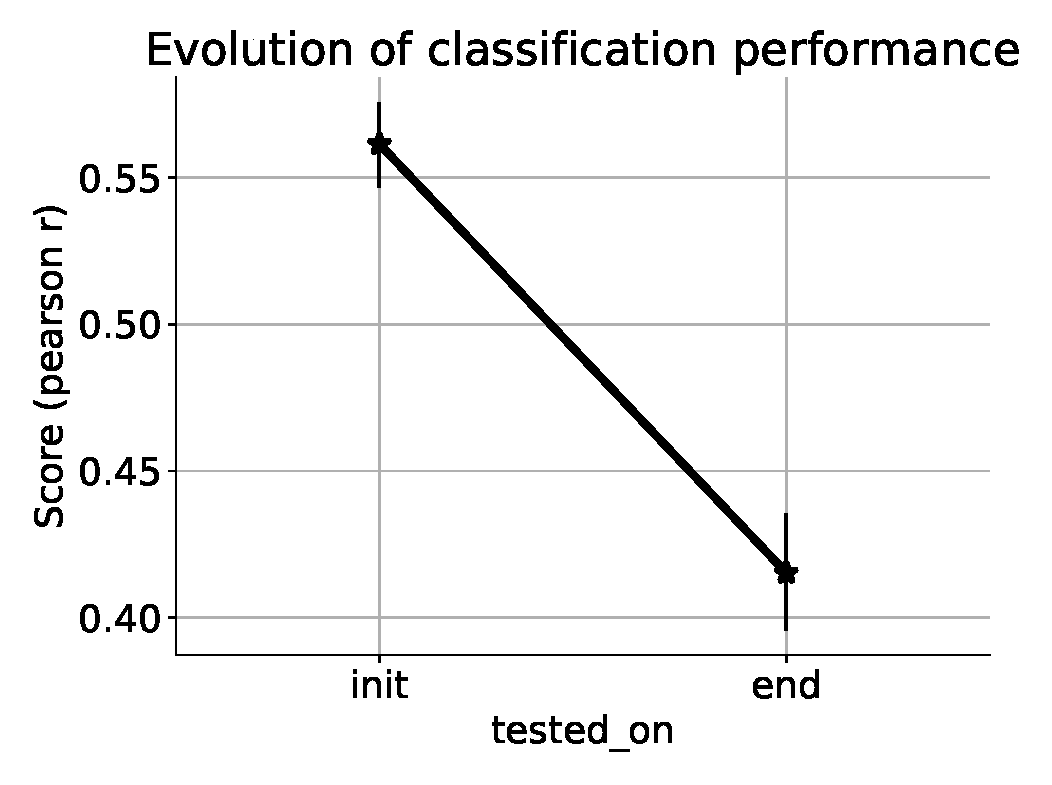
\includegraphics[width=7cm]{figures/PFC_init_vs_end.eps}
    & 
    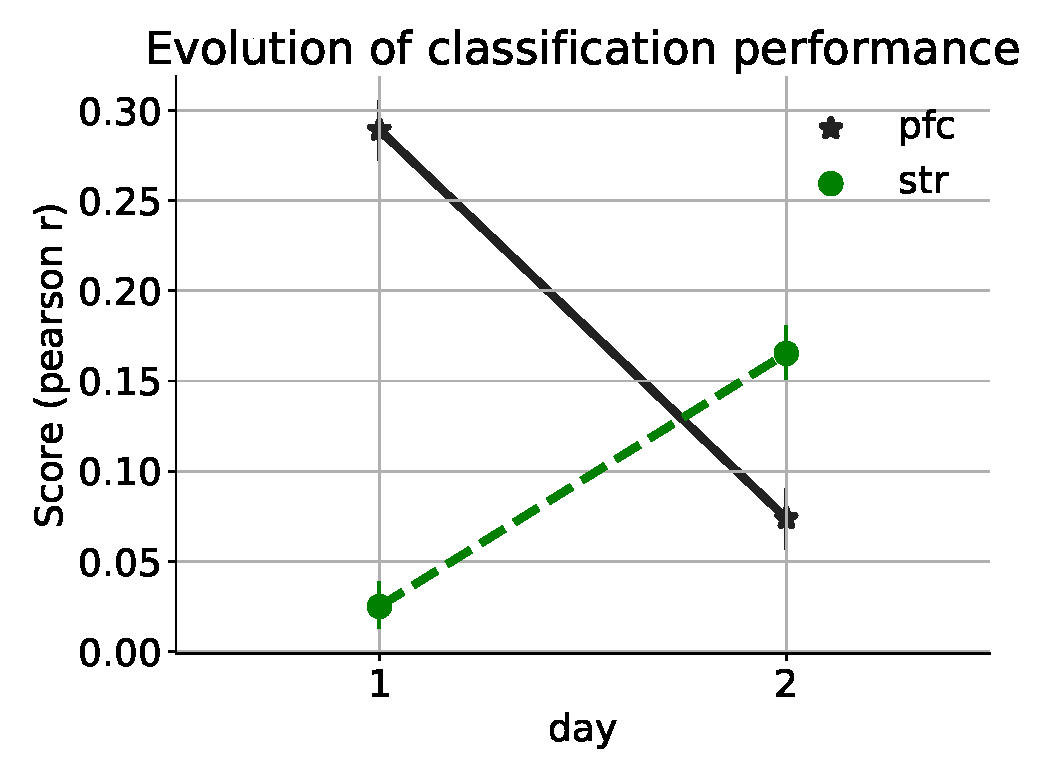
\includegraphics[width=7cm]{figures/STR_PFC_day1_vs_day2_evo.eps}
    \end{tabular}
    
    \caption[Striatum representation enhancement follows PFC's deterioration]{Striatum representation enhancement follows PFC's deterioration. Left: Group 1 at first vs second half of session. Right: Group 2, in different days.}
    \label{fig:time_representation_str_pfc}
\end{figure}

We discuss how this results relate to the already established Dual Process framework for learning.


This work has three kinds of contribution: 
\begin{enumerate}
    \item Methodology: We provide rationale for method choices, grounded on comparisons made available in the corresponding chapters. 
    
    \item Results: Analysis applied to data from our research group, giving results such as the central one aforementioned, are thorougly discussed.
    
    \item Theory: Contemporary discussions from relevant areas are brought in, and the work contextualized in multiple levels.
\end{enumerate}


% 1 paragraph discussion
% 1 small paragraph conclusion


\part{Grounds}
%!TEX root = ../dissertation.tex
\begin{savequote}
We don't want to focus on the trees (or their leaves) at the expense of the forest.
\qauthor{Douglas R. Hofstadter}
\end{savequote}

\chapter{The Brain}
\label{cap:thebrain}

The sensory apparatus of single cell organisms is directly linked to their motor apparatus, meaning that structures capable of detecting perturbations are tightly coupled to structures capable of generating movement \cite[p.~149]{maturana1987tree}. In protozoa, for example, the same flagellum that moves it in the environment also detects obstacles, while some bacteria have chemotaxing mechanisms that change direction of movement, increasing or reducing tumbling rate, in direct response to changes in sugar concentration \cite[p.~147-149]{maturana1987tree}. The coupling between sensory and motor surfaces (i.e. what to do in response to perceived environment), in these direct links, is inflexible.

In contrast to direct sensory-motor connections, the nervous system appears as an intermediate component between the surfaces of interaction of an organism with the surrounding environment. A nervous system endows its owner with structural plasticity, thus enabling learning via changes in this intermediate step between sensory and motor surfaces, producing bigger behavioral repertoires and complex behavior \cite[p.~175]{maturana1987tree}. This comes at the expense of a lot of energy: up to 20\% of human total resting metabolism \cite{attwell2001energy}, which is used mainly by \textit{neurons} \cite{zhu2012quantitative}, a cell type that receives, modulates, and sends signals. The reason why so much of our energy budget is directed towards this single type of cell, can possibly be explained by the importance of its activity for the organism.

With the intermediate system increasing in size, the motor output gets farther apart from the sensory input. The motor output, or behavior, is still conditioned in the organism's perception of the environment, but now abstractions away from the sensory apparatus. On the one hand, some environment characteristics such as a predator's smell or presence of a hurtful shock may have direct impact on behavior. Other ones, such as the identity of objects or the passage of time, may need to be abstracted from the raw sensory input. The specific way in which nervous systems, and in special the brain, produce or develop representations of these environment characteristics to guide behavior, is a central question since the creation of neuroscience.

\textcolor{red}{Here we are missing a paragraph. Why did you say all these things above. You may want to say that they were your inspiration for the study, for getting in neuroscience? The statements above are fairly genneral, so you need a connection to what you are going to say next... }

The introduction was divided into three chapters. In this first, we gave a high-level view of some of the neuroscience challenges and techniques to tackle them, along with the framework that encompasses the rest of the dissertation. In chapter \ref{chap:timing} we characterize the field of \textit{timing}, that encircles and motivates our questions. At last, in chapter \ref{chap:where} we close into our specific motivations and objectives.

\section{What the brain really does}
\label{sec:theory}
    We know that the nervous system mediates the interaction between a living system's sensory inputs, i.e., what is perceived from the environment, and the system's output, e.g., movement. Based only on excitatory and inhibitory connections between neurons, even in the simplest unidirectional case, it is possible to generate reasonably complex behaviors, which can be interpreted as fear responses, aggression, or even logic \cite{braitenberg1986vehicles}. % Possivelmente uma imagem do vehicles, tipo figura 5 pg13
    
    In extremely simple circuits, such as the ones described above, it may be possible to generate mechanistic accounts of this mediation, providing an effective explanation to phenomena like reflex arcs. With little complexity added, these explanations can get really intricate, as in the case of the much-studied Somatogastric Ganglion (STG) of the lobster. The gastric circuit within the STG generates complex oscillatory patterns with a circuit of only 11 neurons \cite{selverston2009neural}. Despite this circuit's smallness, it took 30 years from their discovery to the development of mechanistic explanations for its functions \cite{bal1988pyloric, selverston2009neural}. Also, there are multiple combinations of connections between neurons that give rise to the same rhythms, many of which  found \textit{in natura} \cite{prinz2004similar}. % https://www.nature.com/articles/nn1352
    This raises an important issue in modern neuroscience, viz. that if we want to increase the predictive power of our models, we have to step away from the implementational level, and delve deeper into theories of brain function and general properties of brain activity \cite{gerstner2012theory}. One remarkable proponent of this formalism is the Free Energy Principle \cite{friston2009free}: it states how self-organizing systems -- in particular the brain -- can resist the tendency to disorder. According to the Free Energy Principle, to maintain itself in the narrow band of states that are consistent with physiological bounds, an organism must have an internal representation of the environment, regularly updated by new evidence \cite{friston2009free}.

\section{Levels of analysis}
    There are multiple manners of studying cognition and the brain function beyond the search for neural correlates. To enable these studies to advance, in despite of technical limitations, Chomsky proposed we should develop cognitive models without regard to biological implementation - even though these mechanisms should be worked out at a later stage \cite[p.~12]{chomsky2006language}.

    The necessity to divide the study of the nervous system into levels of analysis took some time to be established. The most prominent division has been proposed by Marr, in the early 80s \cite{leopoldo2018computational}. Confronting limitations of finding neural correlates for divers phenomena, Marr articulates how -- even if we did found the "apocryphal grandmother cell" --, it would not tell us "why or even how such a thing may be constructed from the outputs of previously discovered cells" \cite[p~15]{marr1982vision}. It is true that much has changed since then, especially with respect to the understanding of \textit{how}\footnote{In the case of vision, derivatives from the distributed processing framework eventually gave rise to algorithmic models of the visual cortex \cite{fukushima1980neocognitron}, and the building up of complex cells from simpler ones is now understood and emulated \cite[p~9]{goodfellow2016deep}.}, but Marr's case is clear: multiple characterizations are needed to account for brain operation. 

    \begin{quote}
        The key observation is that neurophysiology and psychophysics have as their business to \textit{describe} the behavior of cells or of subjects but not to \textit{explain} such behavior. What are the problems in doing it that need explaining, and at what level of description should such explanations be sought? - David Marr \cite{marr1982vision}
    \end{quote}

    To understand a particular brain function, it does not suffice to understand its hardware implementation i.e., the neuronal activity and connections. First of all it is necessary to have a precise understanding of what is to be computed. This knowledge makes possible to devise representations and algorithms that are sufficient to compute what is needed, and at last biological mechanisms that implement those algorithms and representations. The levels are not detached from one another, but they are only loosely related. For the reason that explanation for some specific empirical data may come from one single level, as exemplified below.
    
    Time perception in humans is biased: when intervals are reproduced, they tend to regress to the mean \cite{jazayeri2010temporal}. This means that long intervals are reproduced shorter and short intervals are reproduced longer. This finding can be explained in the level of the algorithm: a bayesian algorithm has the same biases, consequence of prior distributions learned across all time intervals \cite{jazayeri2010temporal}. This makes no reference to the specific neuronal circuits recruited to the task. 

    \begin{table}[]
        \centering
        \begin{tabular}{p{4cm}p{4cm}p{4cm}}
        \hline \vspace{.2cm}
            Computational Theory & Representation and algorithm & Hardware implementation\\\hline
            
            What is the goal of the computation, why is it appropriate, and what is the logic of the strategy by which it can be carried out? & 
            
            How can this computational theory be implemented? In particular, what is the representation for the input and output, and what is the algorithm for the transformation? &
            
            How can the representation and algorithm be realized physically?
            \\\hline
        \end{tabular}
        \caption{The three levels at which any machine carrying out an information-processing task must be understood. From \cite{marr1982vision}, figure 1-4}
        \label{tab:three_levels}
    \end{table}
    
    Marr advocates that we need a Computational understanding of a system to conduct the lower level investigations. In the case of vision, he proposed the computational role of "extracting invariant representations", building upon the preceding work that had just started discussing the separation of reflectance and illumination by the visual system, and how this could be accomplished. It is a change of perspective from "what may the system be doing" to "how may the system do this".
    
   
    
        Marr illustrates the framework by the example of a cash register that does the process of addition. This process: 1) maps two symbols into a single one; 2) has rules such as commutativity and associativity, that ensure the process is not affected by ordering; 3) has an inverse and null elements, allowing to subtract quantities or keep them the same. The rationale for these rules is obvious in a setting such as a cash register, where we want no effect of the product ordering, and want to pay nothing if we take nothing. This concludes the computational role of the cash register: explaining \textit{what} it does and \textit{why}, and being "true no matter how the numbers are written -- whether in binary, Arabic, or Roman representation."
        
        The second level explains \textit{how} such a function is performed in the system, from the choice of representation to the algorithm performed using this representation. Both are codependent: specific representations facilitate the use of some specific algorithm and hinder the use of other. Roman numerals, for example, can be used to represent numbers, but they make addition harder (let alone multiplication). The cash register, in Marr's time, used decimal representation for the numbers, the same algorithm that is used by students in basic school, going digit-by-digit from right to left and carrying digits. Wiring and transistors can implement the same representation and algorithm that is implemented by ink and paper.
        
        Finally, we get to the lower level, in the sense of the specific hardware in which is implemented the algorithm that performs the function. This is the level where most neuroscience research focuses, to the point of asking questions such as what are the possible functions performed by some neural circuitry, or in which way neurons could perform some specific function.
    
    % \subsection{Computational models in neuroscience}
        
    %     Models in the computational level have a specific sense in this framework. They define precisely the 
    %     % FEP
    %     % Outros existem?
    %     % Reinforcement Learning
        
    %     For timing, 
        
    %     Recently, the biggest contributor to Marr's ideas, Tomaso Poggio, proposed that we should add two levels of explanation to the original three. The level of \textit{learning} should explain how a given function and representation is developed by an organism, and \textit{evolution} should explain how this learning came to be \cite{poggio2012levels}. 
        
        % \cite{leopoldo2018computational}

\section{Measurements}
    Neurons communicate via synapses, where action potentials in the pre-synaptic neuron trigger the release of signaling molecules (neurotransmitters) that it will directly or indirectly change the electrical potential of the post-synaptic neuron \cite{purves2014neuroscience}. This change is generally due to the activity of ion channels in the cell's membrane \cite{purves2014neuroscience}, and causes changes in the electrical potential between inside and outside the cell \cite{purves2014neuroscience}, creating dipoles and thus electric fields in the region.
    
    % Neurons fire action potentials when their membrane is depolarized enough to open voltage-dependent ion channels. 
    When measuring the electric potential from afar (e.g. using EEG in the scalp), only the summed activity of huge collectives of neurons acting in synchrony can be detected, making it is hard to pinpoint the origin of the signal \cite{buzsaki2012origin}. On the other hand, intracranial electrodes can be placed inside regions of interest in the brain, to detect changes in the electric field in the scale of millimeters and microsseconds \cite{}. The measured activity is then, when high-frequencies are removed, called the Local Field Potential (LFP), and contains information about the collective activity of aggregates of neurons \cite{buzsaki2012origin}. From the high frequencies, we can extract the activity from individual neurons, in specific locations. To this end we use a process named spike-sorting \cite{rey2015past} that extracts the times of action potentials from the voltage timeseries of each electrode. 
    
    The firing of a neuron usually depends on unobservable activity and inner states, such as concentration of proteins \cite{}, and more generally short-term plasticity \cite{motanis2018short}. This makes the sequence of action potentials that are caused by some event to vary from trial to trial, even in cases where the neuron has a known tuning to the event \cite[p~7-8]{dayan2001theoretical}. To account for this lack of knowledge, neural activity is treated probabilistically, by switching from the spike times to the underlying firing rate \cite[p~9-11]{dayan2001theoretical}. The firing rate can be calculated by counting the spikes in sliding windows, or using kernel convolutions, as for example the Gaussian kernel ~\cite[p~9-11]{dayan2001theoretical}.
    
    \subsection{Machine Learning}
        Although the very early days of machine learning are deeply intertwined with neuroscience \cite{mcclelland1986parallel}, univariate techniques prevailed so far in neuroscience studies. Recently, the surge of multi-voxel pattern analysis (MVPA) in fMRI brought machine learning back into the field, later rebranded as Multi-Variate Pattern Analysis and finding ever more applications \cite{haxby2012multivariate}. For more examples and a more thorough explanation about the underlying mathematics, see the appendix \ref{app:ml}. Here we present some examples, including applications in neuroscience.
        
        Machine learning is an active research field, with many techniques aimed at multivariate problems. The kind used in MVPA \cite{merchant2008we}, and the most frequently used in neuroscience, is the Supervised Learning (see the Appendix \ref{app:ml} for a more thorough presentation). Supervised learning aims to disclose - or \textit{predict} - some hidden attribute of data points based on observable attributes  (or features). It predicts the objects contained in an image, based on the values of the pixels \cite{}; it predicts if a given email is spam given the text in the email; it predicts if a given tumor is malignant or benign based on quantitative features.
        
        \begin{figure}
            \centering
            \begin{tabular}{cc}
            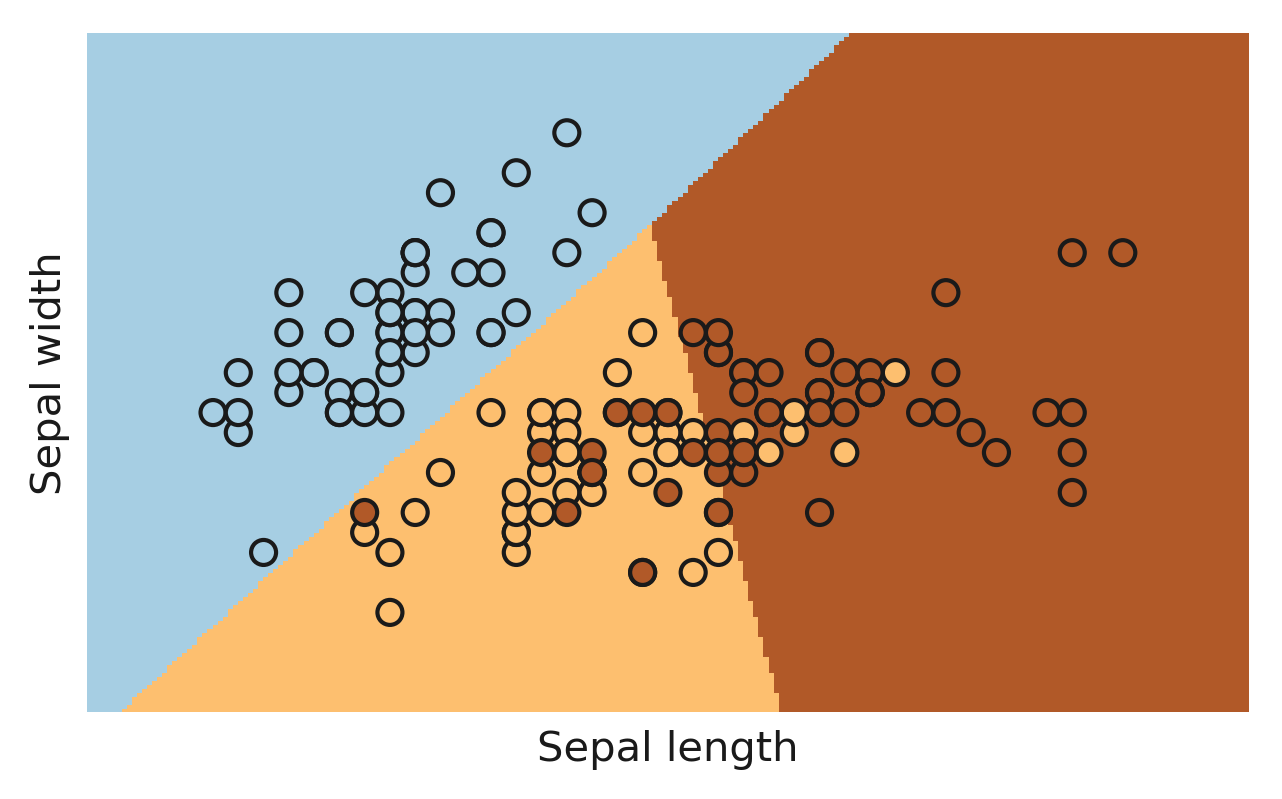
\includegraphics[height=0.33\textwidth]{figures/iris_classification.png} &  
            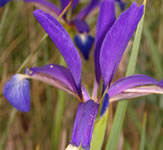
\includegraphics[height=0.3\textwidth]{figures/sketches/Large53.jpg}
            \\
            \end{tabular}
            
            \caption[Classification of the iris dataset]{Classification of the iris dataset into three distinct species, based on two features (sepal length and sepal width). Each circle represents a distinct example (i.e. a flower), and its color represents its species. The classifier linearly separates the plane, and the background coloring corresponds to the classifier's prediction for that location in the plane. Circles that are enclosed in a background distinct from them are erroneous predictions.}
            \label{fig:iris_prediction}
        \end{figure}
        
        We can predict the species of a plant (the attribute) based on sepal and petal length and width. This is a classical example, based on the Iris Dataset \cite{fisher1936use}, and represented in figure \ref{fig:iris_prediction}. The classifier is defined as a mapping from any point in the multidimensional space into a vector of probabilities, with a probability for each possible species. An example of plant, with its feature vector, has then an associated most-probable species, that is given as the prediction of the classifier for that data point.
        
        In neuroscience, machine learning has been generally used in conjunction with other statistical techniques to test hypothesis about the underlying attributes in the neural activity. For example: To test whether activity in the visual cortex contains information about a given stimulus, machine learning can be used to predict the stimulus based on the activity \cite{vetter2014decoding}. If predictions are above chance level, then there was information contained in the activity. Moreover, machine learning methods can be used to compare distinct regions, contrasting of their decoding performance and pattern of responses, as exemplified below.
        
        \begin{figure}
            \centering
            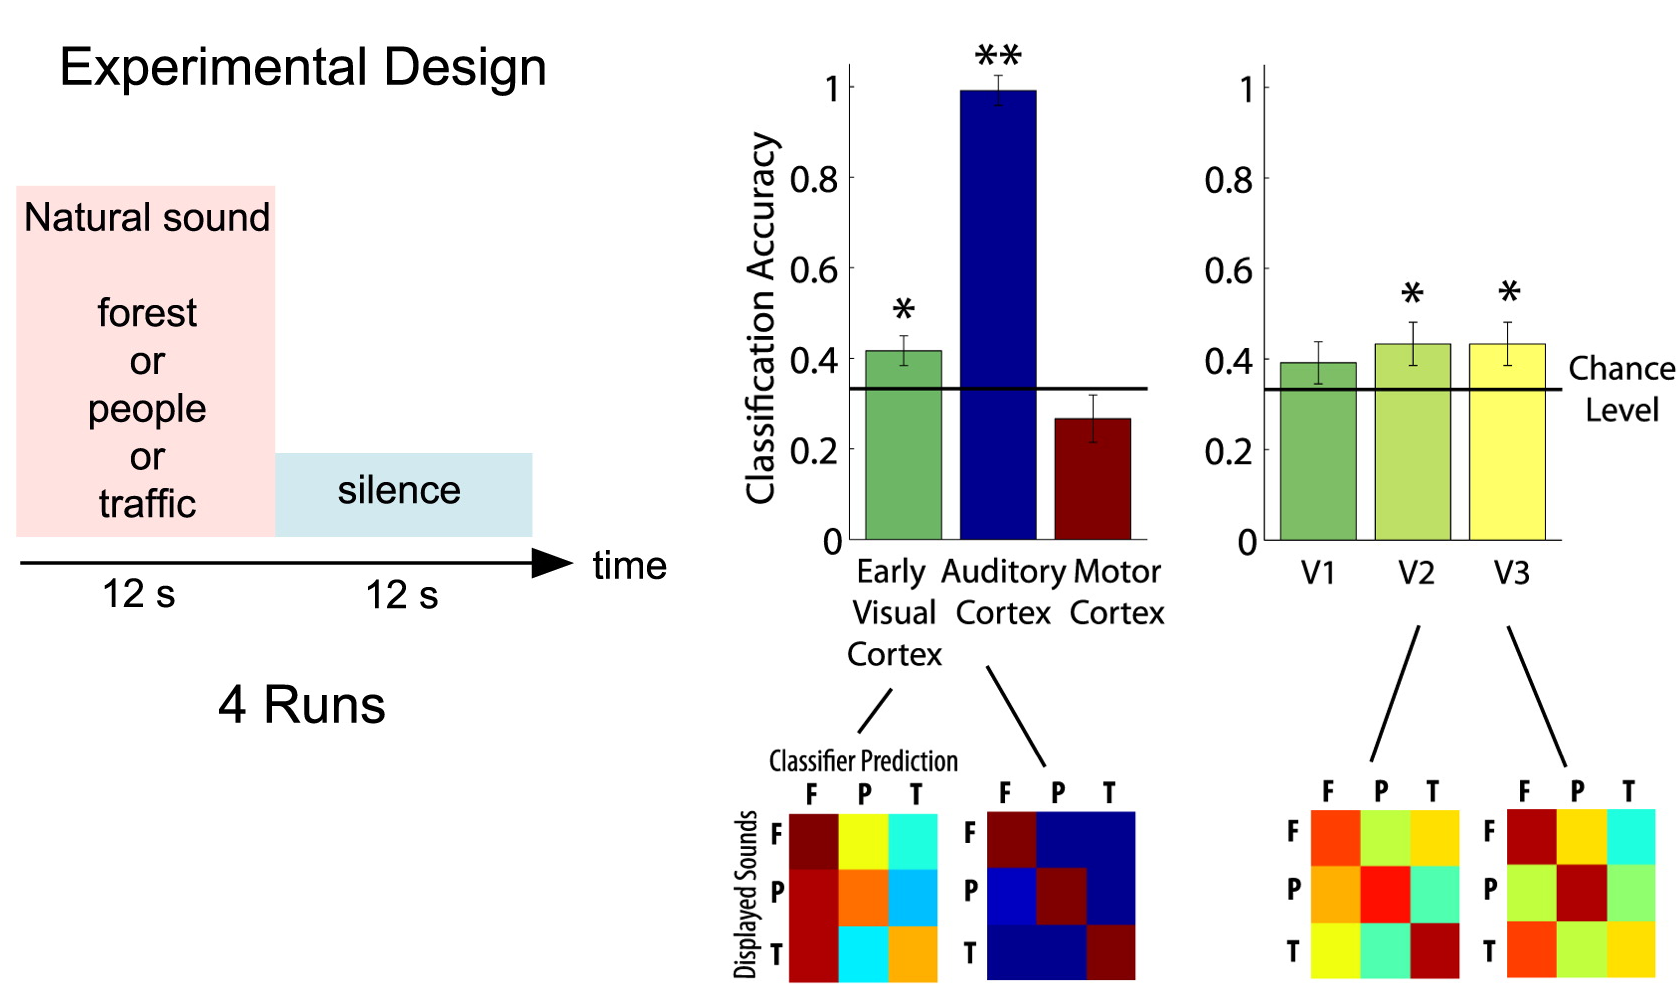
\includegraphics[width=\textwidth]{figures/sketches/sound_prediction_tiny.png}
            \caption[Decoding sound from visual cortex]{Decoding sound from visual cortex. The image shows the design and results for a single experiment using MVPA. A sound is presented, sampled from one of three distinct types of natural sounds, and the subsequent neural activity is fed into a classifier that tries to predict the sound. In the bar plots, the accuracy of classifier predictions is measured for each brain region. Neural activity from three regions is compared, and for three subregions inside the early visual cortex. The heatmaps in the bottom are confusion matrices, that show the count of predictions for each possible combination of displayed sound and predicted sound. Adapted from Vetter et al.~\cite{vetter2014decoding}.}
            \label{fig:prediction_neuro}
        \end{figure}
        
        In figure \ref{fig:prediction_neuro}, Vetter et al. \cite{vetter2014decoding} used machine learning to assess whether multiple regions encoded information about auditory stimuli. After decoding presented sounds (the hidden attribute) from the neural activity of each region, they tested whether the decoding performance was above chance. The predictions were accurate for the auditory cortex, what is not a surprise. A more surprising result was that the early visual cortex also performed above chance. Analyzing more specifically, they showed that this information was mainly on V2 and V3 cortices, and V1 alone did not perform above chance. Vetter et al. presented four other experiments and results to demonstrate that the brain can translate abstract information to encode in the early visual cortex \cite{vetter2014decoding}.
        
        One advantage of machine learning techniques is their generality: they make less assumptions than classical analysis. Supervised learning, the kind most used in MVPA, encompasses two main techniques: Regression and Classification. They both tackle the same problem of decoding hidden attributes, but make different assumptions about the encoding. In regression the attribute is considered continuous, while in classification the attribute is one of a set. In both cases, there are many degrees of freedom that are fitted from the data, lessening the need for domain knowledge about the encoding\footnote{In the machine learning community, domain knowledge about the encoding is usually referred as \textit{feature engineering}.}.

        % \cite{merchant2008we} % MVPA temporal generalization

\section{Representation}
\label{sec:representation}
    The notion that representation is central to cognition is old \cite[p.~134-140]{rosch1991embodied} and it grounds one central method for assessing brain function: the search for neural correlates of measurable quantities. We know that there are neurons in the primary visual cortex that represent (i.e., encode) inclination angles of bars \cite[p.~13]{dayan2001theoretical} and neurons in the primary motor cortex that represent the angle of reaching movements \cite[p.~14]{dayan2001theoretical}. But more complex concepts -- like one's grandmother \cite{gross2002genealogy} or causality \cite{blakemore2001brain} -- may be highly dependant on the context to be captured with such specific correlates.
    
    Since the early days of neuroscience, there is a debate about the general form of brain representation. Cognitivists posed that representation is formed by well defined strings of symbols that logically interact, while connectionists maintained that representation is distributed in the neuronal connections. The former vision is exemplified in the seminal McCulloch \& Pitts paper \cite{mcculloch1943logical}, where they propose that "To each reaction of any neuron there is a corresponding assertion of a simple proposition". The latter is commonly exemplified by modern machine learning \textit{neural networks}, where single neurons rarely have some \textit{meaning} on their own. Connectionism gained strength in the late 80's by the seminal Parallel Distributed Processing \cite{mcclelland1986parallel}, and although many of its related algorithms fall short of biological plausibility, there are those such as Hopfield Networks and Boltzmann Machines, based on autoassociative rules reminiscent of Hebbian learning, that made their way into modern models of brain function \cite{mceliece1987capacity}. 

    The debate between Cognitivism and Connectionism cuts across levels of analysis, making it specially intricate. Implementational connectionists pose that the views are consistent with one another, with the brain's neural network acting as a distributed system that, when analyzed through a higher level of abstraction, is a symbolic processor \cite{bechtel1988connectionism}. Alongside this theoretical studies, measurements of neural activity are generally studied through the lens of representation, with the most prominent being single neuron representations \cite{quiroga2005invariant}, mainly consistent with the Cognitivist view.

    Single neuron representations have been specially studied by the vision community \cite{deyoe1988concurrent, bell1997independent, ito2004representation, lee2008sparse}, but recent contributions have taken this approach much beyond the sensory realm, to the more abstract domains of \textit{space} and \textit{time} \cite{eichenbaum2014time}. \textit{Place cells} are neurons that fire in specific locations of some environment \cite{foster2006reverse}, and are mainly present in the Hippocampus \cite{o1979review}. In the same way, \textit{time cells} fire in specific times after some event \cite{tiganj2016sequential, eichenbaum2014time}, and may serve as temporal basis for representations of the world \cite{ludvig2008stimulus}, being complemented by \textit{ramping neurons}, that linearly increase or decrease their activity during a time interval \cite{morrison2009convergence, kim2013neural, tiganj2016sequential, parker2016timing}.

    %, bestowing the brain with a whole new dimension along which to relate its activity \cite{eichenbaum2014time}

    It becomes clear, through the previous paragraphs, that the search for neural correlates deeply entangles the representational and implementational levels, and may be better understood through some conceptual distancing. Representations have to do with the internal objects that are transformed through some algorithm, for which many implementations are possible. Take the following example: time is a quantity that evolves monotonically and linearly, and so does its representation. The monotonicity can be achieved by any phase-space trajectory, with the condition that it does not cross itself. In addition, linearity can be achieved by a simple nonlinear regression reading-out the monotonic activity. The regression could be implemented having another general trajectory as output \cite{gallant1975nonlinear} or a single ramping neuron: The choice of input and output is by no means obvious, and depend at least as much in the computational goals as the implementational constrains.
    
    Although there are many examples of quantities encoded in single neurons, such as aforementioned, it is not necessary that particular neurons have such interpretable roles. Phase space trajectories can be composed by the activity of populations \cite{shamir2014emerging, quiroga2009extracting}, as well as less explicit dimensions such as post-synaptic sensitivity \cite{motanis2018short}, and neuromodulation effects \cite{friston2009free, friston2010free}. While the latter two also affect behavior \cite{wolff2017dynamic}, we do not account for them in the present work, as they are not directly detectable from neural activity. Hence, the present work focuses in population activity.
    % accumulators bueti2011physiological, wittmann2010accumulation
    
    Population codes have the capacity to carry much more information than single neuron codes \cite{hardy2016neurocomputational}, but since population patterns are by definition multivariate, their study requires more elaborate techniques \cite{quiroga2009extracting}, such as Machine Learning. 
    There are many ways in which a given neural population may encode information \cite{quiroga2009extracting, shamir2014emerging, mello2015scalable}, and we discuss some proposals specific for time in the next chapter.
\chapter{Timing}
\section{What is timing .:}
    Every behavior carries out through time, and in special any motor action has an execution time, but the study of timing is not so generic: to say that an animal is timing isn't simply because its behavior occurs in a certain time. Machado \cite{machado2009learning} proposes the animal is timing when "the best predictor of its behavior is an interval of time", a definition that narrows the domain, but emphasizes the observer in despite of the computation being performed. In addition, there are well-established timing processes that fall short of this definition by being parts of some bigger computation and not directly effectors of behavior. Although there is no consensus on a precise definition of what is timing in a computational sense, the notions of "telling time" \cite{}, and structuring events and processes with respect to time \cite{} are enough to characterize a wide range of processes.
    
    Mechanisms for measuring time are found in a variety of organisms, from humans to plants \cite{cashmore2003cryptochromes}. Initially bound by external rhythms (like circadian cycles), time estimation mechanisms were among the first competencies evolved in biological systems \cite{paranjpe2005evolution}, and are constitutive of many other cognitive modalities such as decision making and episodic memory \cite{maniadakis2014time}. Most behavior is inseparable from a temporal or rhythmic component \cite{buhusi2005makes}. From deciding to accelerate or break in a yellow light, through the simple motor organization of walking or running, to the complex dynamics of speech and musical performance, computational processes are temporally structured to correct execution \cite{bueti2014temporal}. 
    
    While organisms and their brains have to account for event durations in many timescales, from milliseconds to days, there is no single neural correlate able to account for them all \cite{buhusi2005makes, buhusi2016clocks, hardy2016neurocomputational, lewis2003distinct, mauk2004neural}. On the one hand, circadian rhythms depend on the suprachiasmatic nucleus (SCN), relying on slow protein cycles managed by transcriptional feedback loops \cite{buhusi2005makes}, and are important to regulate social and foraging behavior. In turn, the temporal structure of milliseconds relies on local circuits and their communication with the cerebellum \cite{ohmae2017cerebellar}, and is essential to fine motor control, such as playing an instrument or making a tool. In between, the time scale of seconds is central to planning, decision making and reasoning \cite{buhusi2005makes}, and is dependent on the Striatum \cite{mello2015scalable}, but independent of the SCN \cite{lewis2003interval}, and cerebellum \cite{harrington2004does}. The present work focuses in the scale of seconds, named as \textit{interval timing}.
    
    The scale of seconds is less well-understood than its counterparts, but there is much experimental evidence about regions and mechanisms involved in its estimation. Evidence comes from a variety of sources, from psychophysics \cite{ohmae2017cerebellar} and pharmacology \cite{pine2010dopamine, meck2012gene, drew2003effects, cheng2016clock, ludvig2008stimulus} to lesion studies \cite{} and electrophysiology \cite{bakhurin2017differential}. From psychophysics, we know that time estimation obeys Weber's law \cite{gibbon1977scalar}, meaning that the error is proportional to the mean, and thus time-scale invariant; From pharmacology, we know that dopamine agonists shorten time estimates while antagonists elongate them \cite{}; Lesion studies show some regions necessary for timing behavior \cite{};
    Lastly, electrophysiology shows neural correlates of timing \cite{}.
    
    In the rest of this chapter we will present two complementary ways of characterizing 
    
    
\section{Timing models}
\label{sec:models}
    The Scalar Expectancy Theory (SET) proposes a model, schematized in figure \ref{fig:set_schema} where timing is achieved by a counter, that accumulates pulses from a pacemaker and compares them with reference memories \cite{}. Despite the simplicity, the model fits psychophysical data from the most common timing tasks \cite{} correctly predicting time-scale invariance, and can explain the effect of dopamine as simply an accelerator of the pacemaker. 
    
    \begin{figure}
        \centering
        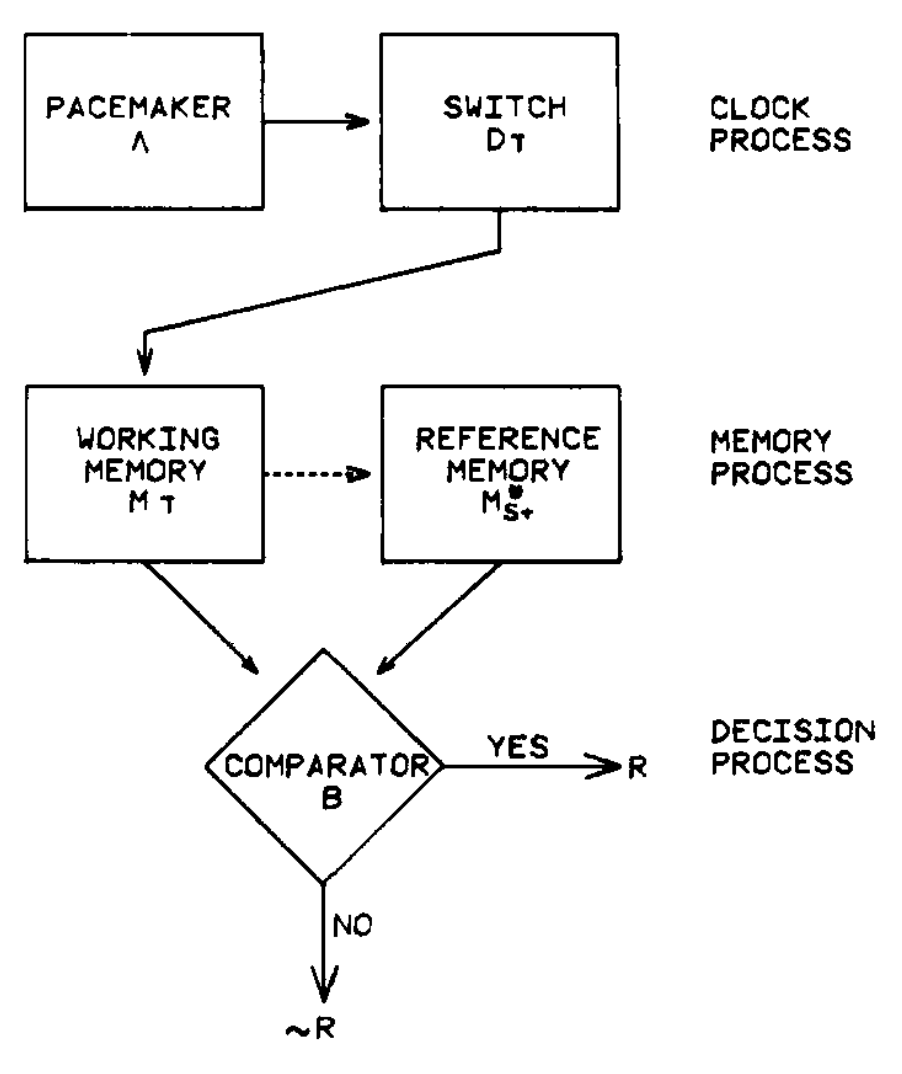
\includegraphics[width=5cm]{figures/SET_model_schema.png}
        \caption{Caption}
        \label{fig:set_schema}
    \end{figure}
    
    The SET model is by far the most popular timing model \cite{}, having retained attention from the community for more than 30 years. Even though it has limitations and fails to predict some results \cite{machado2009learning}, its simplicity seems to compensate for it. There are too many timing models to consider an exhaustive listing \cite{}, and we introduce those that best foster our examination across levels of analysis. 
    
    In terms of algorithm, it has been shown that Drift Diffusion Models (DDMs) are a more general framework that encompasses the SET, LET, and other common models \cite{balci2016decision}. DDMs are evidence-accumulation models, that compare the evidence among two alternatives in a noisy setting, and are optimal in the sense they can reach some predetermined accuracy in the least amount of time. They have the interesting uptick of being commonly used to study decision making, and thus frame timing in terms of decision. 
    
    At the level of implementation, the most discussed model is simply the ramping neuron \cite{}, where single neurons increase their activity up to a threshold that triggers the response. Single neuron models also feature time cells \cite{}, whose activity marks a point in time. Alternatively, there are a variety of state-dependent network models (SDNs) \cite{}, where time is represented in the collective activity of many neurons \cite{}. In the halfway, "synfire chains" model sequentially activated cell assemblies \cite{}. From these examples, state-dependent networks are the most general: all of the other models can be interpreted as SDNs \cite{}. However, instances of SDN proposed in the literature generally emphasize that trajectories in the phase space are intricate, in opposition to the elementary ones that could be represented by the simpler models \cite{}.

    There are many attempts to bridge the gap between Algorithm and Implementation, one of which is proposed by Simen et al. \cite{}. They build up from individual neurons to a DDM, by successive approximations, going through two steps of neural populations.
    
    \subsection{Intrinsic vs Dedicated}
        %Ler
        Among models of timing, there is an ongoing discussion on the intrinsicness of the processes involved in timing. While much of the discussion around time processing has 
% Converging data supports intrinsic models
\section{The taxonomy of timing}
\label{sub:taxonomy}

    The split between explicit and implicit memory was a breakthrough, providing a framework that enabled new kinds of questions \cite{paton2018neural}. % Change, explain
    
    % The scale of seconds has a name, but not clear boundaries. What constitutes interval timing may range from seconds to hours in some studies \cite{}, and from tens of milliseconds to seconds in others \cite{}. 
    
    The field of timing currently lacks a thorough taxonomy, grouping forms of timing that depend on similar circuits and mechanisms \cite{}, and distinguishing those that do not. Paton and Buonomano \cite{paton2018neural} proposed one such grouping, to be used as starting point in this endeavor. They considered the computational requirements of many tasks, and arrived at a three-dimensional account for them
    \begin{enumerate}
        \item \textit{Subsecond vc Suprasecond timing}. The most established dimension along with timing tasks vary, it is
        \item \textit{Motor vs Sensory timing}.
        \item \textit{Interval vs Pattern timing}.
    \end{enumerate}
    

    In a meta-analysis of fMRI timing studies, Lewis and Miall \cite{lewis2003distinct} proposed three dimensions that, in tandem, could split tasks into two groups with distinct neural substrates. The first group is Automatic Timing, dependent on motor and sensory circuitry such as \ac{m1}, \ac{s1} and \ac{sma}, and the second is Cognitively Controlled Timing, dependent on regions of the \ac{pfc} and \ac{ips}, among others. The dimensions proposed, enough to distinguish the two task groups, were the following:
    \begin{enumerate}
        \item \textit{Interval size}. Long intervals tend to require cognitively controlled timing.
        \item \textit{Presence of movement}. Movement eases the use of automatic systems for timing.
        \item \textit{Continuity/predictability}. When intervals are measured in a repeating cycle or in a predictable pattern, less            attention is required by the task and thus it may be tackled by the automatic system.
    \end{enumerate}
    The dimensions they proposed map almost fully into those recently proposed by Buonomano, with the major distinction being that they propose a principal component of variation, from automatic to cognitively controlled. 
    
    \begin{figure}
        \centering
        % \includegraphics{}
        \caption{Automaticity as a composite dimension.}
        \label{fig:automaticity}
    \end{figure}
    
    % \Paragraph Explain mapping between dimensions
    
    % \Paragraph Why it is important to distinguish mechanisms
    
    % \Paragraph importance of learning
    % how our understanding of learning may increase our caspacity to taxonomy timing?

    % maybe 

\section{The anatomy of timing}
\label{sub:anatomy}
    
 % talvez caiba melhor na discussão
    The scale of time intervals is widely used as distinction between experiments \cite{van20168, buhusi2005makes, hardy2016neurocomputational}, and commonly considered sufficient to characterize timing tasks \cite{buhusi2005makes}. Accordingly, the scale of seconds to minutes is called \textit{Interval Timing}, and its characteristics are assessed through several tasks \cite{lloyd2012neural,astrand2014comparison,brea2016prospective,mello2015scalable,gouvea2015striatal,kopec2018controlling,gershman2014dopamine,tiganj2016sequential,narayanan2009delay,cho2010differential}. While neural structures necessary for good performance differ among Interval Timing tasks \cite{paton2018neural}, there may exist a single neural mechanism rendering the time representation \cite{gibbon1977scalar}, or still further a single region for Interval Timing common to all of them \cite{mello2015scalable}. Some common properties detected across tasks support this idea of a single mechanism underpinning all timing in the order of seconds \cite{buhusi2005makes, gibbon1977scalar}. The scalar property is the fact that errors in the time estimation are  proportional to the interval being estimated \cite{oprisan2014all}, and it is present as a feature of many models \cite{gibbon1977scalar, oprisan2014all}. The dependence on dopamine to its correct performance is also characteristic of Interval Timing tasks \cite{kim2017optogenetic, meck2012gene} -- excess of dopamine causes underestimation of intervals \cite{cheng2016clock, pine2010dopamine}, while lack of dopamine leads to their overestimation \cite{drew2003effects}. 
    
    Independently of how dedicated or intrinsic are time representations, an important role is traced to cortico-striatal circuits \cite{lusk2016utilizing, buhusi2005makes, meck2008cortico}, in special to the mPFC \cite{buhusi2018inactivation} and the Striatum \cite{mello2015scalable}.
        
    \subsection{Medial Pre-Frontal Cortex}
    % TODO anatomy
    % TODO connections
    % TODO functions
        The medial prefrontal cortex has been implicated in Timing in multiple tasks, such as Reaction Time \cite{narayanan2009delay}, Differential Reinforcement of Low rate \cite{cho2010differential} Temporal Bisection \cite{kim2009inactivation,tiganj2016sequential,kim2013neural}, and Peak Procedure \cite{buhusi2018inactivation}, by distinct methods such as lesions \cite{cho2010differential}, inactivation by muscimol \cite{buhusi2018inactivation, kim2009inactivation}, and optogenetic stimulation \cite{kim2017optogenetic}.
    % TODO timing
        
        
    \subsection{Striatum}
    % TODO anatomy
        The Striatum is a part of the basal ganglia, a series of nuclei that connect both to Cortex and Brainstem \cite{helie2015learning}. 
    % TODO connections
    % TODO functions
        Its traditional roles relate to procedural learning, and to the initiation and termination of movements \cite{helie2015learning}. Deficiencies in the basal ganglia might cause diseases like Parkinson's, in which patients' erratic movements and tremblings show deregulation of movements' bounds by lack of dopamine \cite{buhusi2005makes}. An intact Striatum is required for performing many Interval Timing tasks \cite{mello2015scalable,gouvea2015striatal,cho2010differential}, such that it is the centerpiece of many timing models \cite{mello2015scalable, buhusi2005makes}.
    % TODO timing
    
        While much has been done in the context of timing performance, the mechanisms through which the correct behavior develops during learning are much less studied \cite{van20168}.

\chapter{Instrumental and Reinforcement Learning}


\section{Learning to Time}
While most of the work in Timing has focused on well-trained subjects \cite{}, the current most discussed models of timing make explicit mechanisms for learning, that until now have been assessed mostly via the biases imposed after training \cite{}

\section{}



\chapter{Where we are}
\section{}


\part{Methodology}
\chapter{Objectives and Hypothesis}
\label{chap:hypothesis}

The current work aims to assess how neural activity changes through learning, with respect to the representation of time. Specifically, our objectives are divided into one methodological and one practical.
\begin{itemize}
    \item Methodological: To understand how the choice of classifier may impact results. Are the results highly dependent on the kind of classifier used for analysis?
    \item Practical: To understand how the quality of representation changes when comparing naive and proficient rats.
\end{itemize}

With respect to the methodology, we expected the choice of classifiers to influence the results as a matter of degree, but not qualitatively. That is: classifiers could each have different performances, but all will be able to find significant patterns.

As to the practical aspect, we expected the quality of time representation to increase as a function of proficiency, as depicted in figure \ref{fig:hip}, which means that after learning the performance of classifiers should increase. 

\begin{figure}
    \centering
    \includegraphics[width=\textwidth]{figuras/hipot.PNG}
    \caption[Visual sketch of our hypothesis.]{Visual sketch of our hypothesis. We expect that when the animal is learning the representation is weak or absent, and is stronger when the animal is performing well.}
    \label{fig:hip}
\end{figure}

\chapter{Experiment description}
\label{chap:experiment}

\section{The task}
The subjects were adult naive male Wistar rats (12 - 16 weeks old, 380 - 400g). The animals were housed individually in a 12h light/dark cycle with the light turned on at 7am, and put under food deprivation to gradually reach and then maintain 85\% of their free-feeding weight. Animals were handled according to the experimental protocol approved by the Committee of Ethics in Animal
Usage from UFABC (CEUA-UFABC). All procedures were conducted during the light cycle.

Animals were trained in a operant chamber developed in our laboratory, totally controlled by an Arduino uno, and made of acrylic plastic. The box has a \textit{nosepoke}, which is a hole equipped with an infrared emitter-sensor that detects when the animal pokes inside. In the same wall there is a drinker coupled to a lickometer, to which the animal has its access limited by a gate controlled by a stepper motor.

\begin{figure}
    \centering
    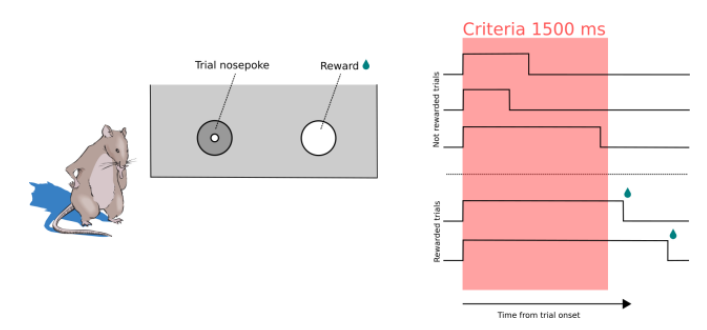
\includegraphics[width=\textwidth]{figuras/methods/tarefa_eli.png}
    \caption[Our DRRD task]{Our DRRD task. If the animal stays in the nosepoke for longer than the criteria, it can collect a reward. Taken with permission from \cite{Eliezyer2018}}
    \label{fig:task}
\end{figure}

\clearpage

First, the animals were shaped to nose poke the hole through a continuous schedule of reinforcement (CR). To conclude this phase the animal had to nose poke the hole at least 100 times on a 60 minutes session. After reaching this performance,
on the next day, the animals were trained with a Differential Reinforcement Response Duration (DRRD) procedure: The trials were self initiated and self ended. In order to receive reward (four licks of a 50\% glucose solution), the animal had to poke the hole and hold for a time equal or longer than the defined criterion of 1500ms. If the animal didn't reach the time criteria there is no reward, and it is free to start a new trial at any time. All sessions were video recorded.
\chapter{Data}
\section{Acquisition}
\label{sec:acquisition}

    Arrays of electrodes were chronically implanted by stereotaxic surgery. For the first group of animals, 32-electrodes array made by TDT (Tucker-DavisTechnologies, EUA) were implanted in the right mPFC (AP: 3.2mm, ML: 1mm, DV: 3.3mm) at UFABC's Electrophysiology lab. For the second group, 32 custom manufactured electrodes were divided, and half implanted on the Dorsal Striatum (AP: 0.28 $\sim$ 2.28 mm, ML: -1.8 $\sim$ -3.5 mm ) and half in the Prefrontal Cortex (AP: 2.52 $\sim$ 4.20 mm ML: -0.3 $\sim$ -1.3 mm). All coordinates were assessed via craniotomy, and measured from the bregma.
    
    The signal was recorded using TDT equipment while the animals were performing the CR or the DRRD task, with a 25KHz rate acquisition. The unit signal was filtered between 1 to 5 kHz. Spike sorting was first performed online and then by the \textit{Open sort} software also developed by TDT. Spike activity was analyzed for all cells that presented the peak of firing rate above 0.1 Hz. 

\begin{table}[htp]
    \centering
    \begin{tabular}{l|l|c|c|c|c|c}
        Animal & Group & Trials & Rewarded & \% Rewarded &  mPFC Neurons & STR Neurons \\\hline
        3 & 2 &  543 / 625  &    278 / 410 &   51 / 65 &       4 / 9    &   10 / 13 \\
        4 & 2 &  436 / 381  &    218 / 222 &  50 / 58  &      25 / 24   &   23 / 11 \\
        5 & 2 &  509 / 437  &    156 / 203 &  30 / 46  &      3 / 5     &   12 / 17 \\
        6 & 2 &  936 / 699  &    404 / 382 &  43 / 54  &      2 / 2     &   0 / 3   \\
        7 & 1 &     1192    &    654       &    54     &     23       &     -     \\
        8 & 1 &      801    &    454       &    56     &     28       &     -     \\
        9 & 1 &      932    &    504       &    54     &     14       &     -     \\
        10& 1 &     1671    &    1030      &    61     &     68       &     -     \\
    \end{tabular}
% \toprule
    \caption[Dataset specifications]{Dataset specifications. The animal's number does not represent any ordering. Group 2's neural activity was measured in two regions, and in two sessions, while group 1's only in the mPFC, and in a single session. The slash in animals of group 2 separate the number of neurons recorded in the first session (at left) from the second session (at right).}
    \label{tab:subjects}
\end{table}
\section{Processing}
\label{chap:processing}

\subsection{Epoching}
    We used the triggering signals from the behavioral box to select the intervals of interest. For each trial, we considered only the spikes that occurred 500 ms before the head-entry was detected -- when the infrared beam of the nosepoke was interrupted -- and those that occurred up to the withdrawal of the nosepoke. 
    
    \begin{figure}
        \centering
        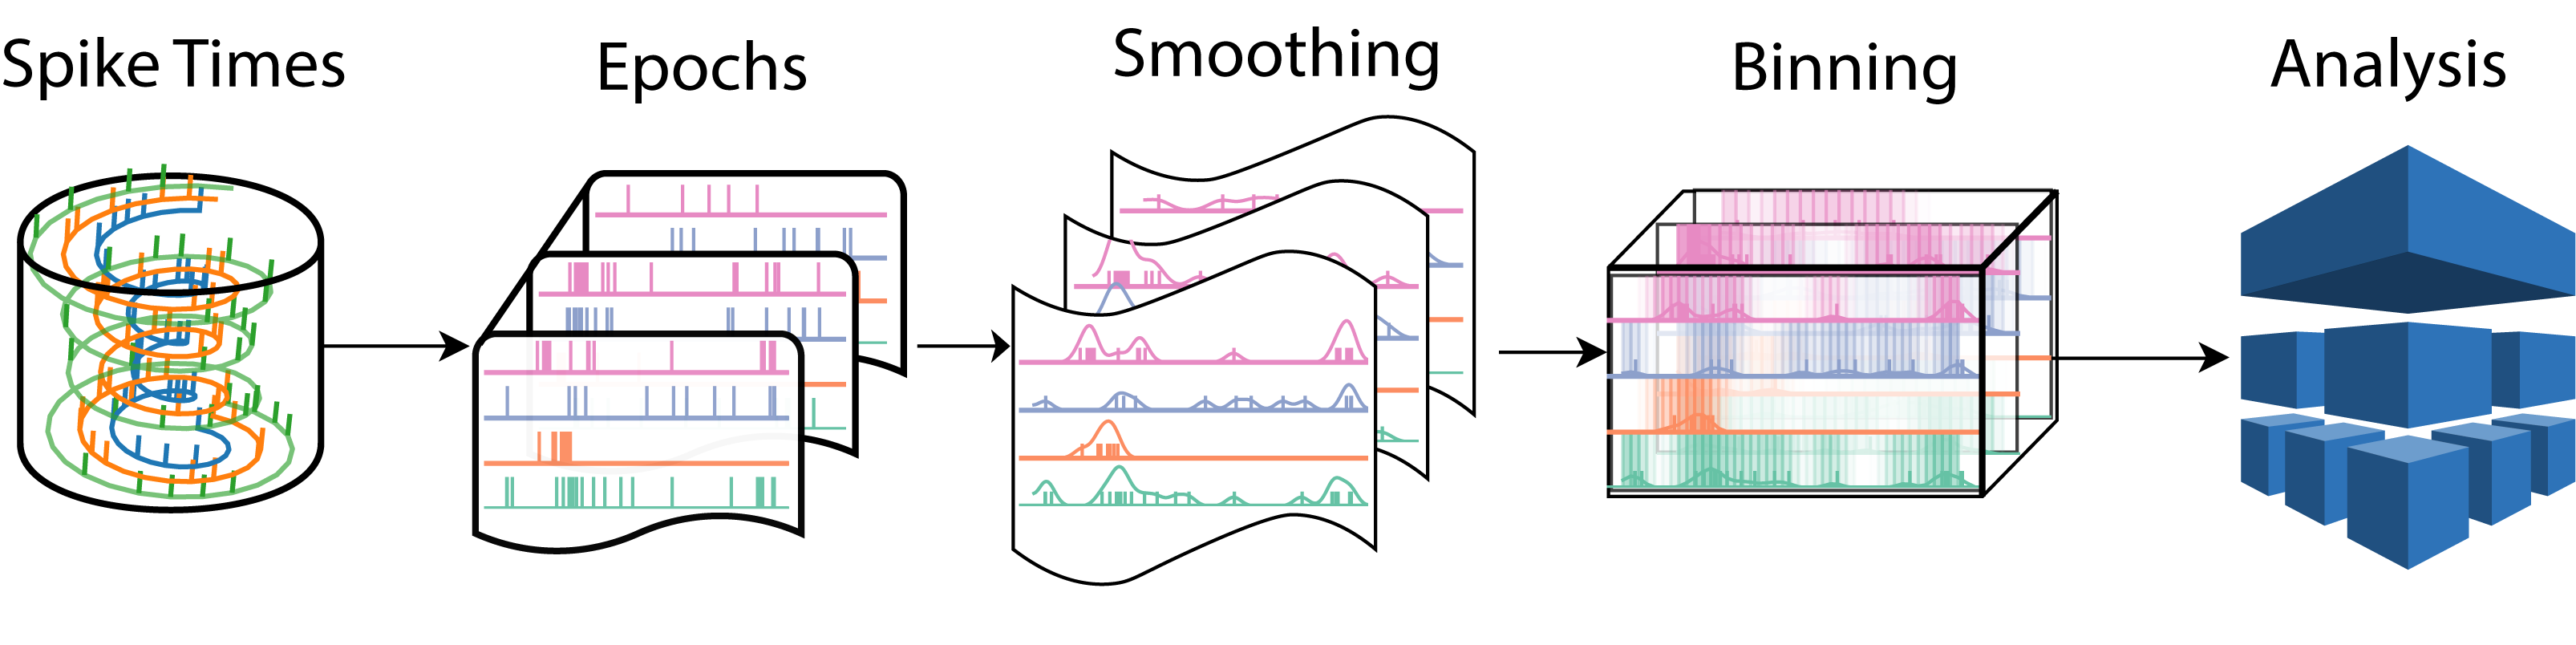
\includegraphics[width=\textwidth]{figures/Pipeline.png}
        \caption[Spike pre-processing steps]{Spike pre-processing steps: Spike times are epoched according to the nosepoke onsets, then smoothed to their estimated firing rate, and finally binned in equal-sized time bins, before being analyzed by machine learning. In the three intermediate steps we can see the activity of four neurons, in three different trials, through the pre-processing steps.}
        \label{fig:preproc}
    \end{figure} 
    
    % We divide spikes into their corresponding trials by using the events measured by our box. For each trial, we get all spikes that occurred between baseline (500ms before trial onset) and trial offset. This means it is possible to have the same spike in two trials, in cases when the intertrial interval is less than the baseline duration of 500ms, which was considered non-problematic.
    % \subsection{Firing rate estimation}
    % Before convolving we have to transform the time stamps into a boolean timeseries, for which we choose the precision of 1ms. Each neuron has then a time series of zeros and ones, with ones in times where the neuron was spiking.e

\subsection{Firing Rate estimation}
\label{subsec:fr_estimation}
    %We transformed the spike time-stamps into firing rates by convolving them with a gaussian \textit{kernel}, with standard deviation $\sigma = 100ms$ and symmetric padding, to avoid creating temporal information which would appear in the case of zero padding. After the convolution, we bin the spikes into windows of 100ms. For a given time bin we have a vector of activity, representing neurons' mean firing rate during those 100ms. Each dimension in this vector represents a different neuron.
    
    %For each trial, we analyze the activity from nosepoke onset until nosepoke removal. Over this interval, the activity from each neuron simultaneously recorded was transformed into firing rate by convolving with a gaussian and then averaging inside bins of 100ms. This procedure resulted in one population firing rate vector per 100 ms time bin, to a total of 15 vectors for 1.5s trials, 30 vectors for 3s trials, and so on. Only the first 15 bins were used for the analysis of bigger trials. 

    For each trial, we analyzed the spike activity from nosepoke onset until nosepoke removal. Within this interval, the activity from each neuron recorded was transformed into a firing rate. This conversion was conducted by convolving each spike with a gaussian \textit{kernel}, of standard deviation $\sigma = 100$~ms and symmetric padding, which avoids introducing artificial temporal information as it happens with zero padding (see Chapter \ref{chap:data_processing}).
    
    After the convolution, we calculate a histogram by counting spikes contained in windows (bins) of 100~ms. For a given time bin we have a vector of activity, representing the average firing rate of neurons during those 100ms. Each coordinate in this vector represents a different neuron. This procedure resulted in one population firing rate vector per 100 ms time bin, to a total of 15 vectors for 1.5s trials, 30 vectors for 3s trials, and so on. Only the first 15 bins were used for the analysis of trials longer than 1.5s.

    % We used three values for the standard deviation (20, 50 and 100), to assess the robustness of our analysis with respect to this parameter. To test the effects of different padding choices in estimating the firing rate, we compared the spike count (not smoothed) in 100ms bins with the firing rates measured using a gaussian kernel with standard deviation of 100ms, calculating the borders with either the default zero padding or a symmetric padding. At last we used the
    %, 50 and 20 ms. While the windows of 100 and 50 can be used for computationally expensive analysis, The window of 20ms is stored for visualization purposes.

\subsection{Disengagement exclusion}
    Inter trial interval, or ITI, is the time between two nosepokes. Specifically, it is the interval from when the animal exits the nosepoke until it enters again.
    The level of engagement was assessed using the inter trial interval of each animal. For such, we calculated the sum of ITIs occurring within a moving window of 5 trials. The first occurrence of a sum bigger than 5 minutes inside a window was defined as the disengagement point. All posterior trials to the disengagement were removed from further analysis.
    
\subsection{Correct trials}
    Unless otherwise specified, we selected as correct trials all rewarded trials (t > 1.5s) for our analysis, after the removal of trials without engagement. 
    
\subsection{Neuron pool}
    As typically done in the literature, we merged cells from all rats in most analysis. Correct trials were ordered and aligned for each group of animals, from the first trial of each animal to the last trial of the animal with the smallest session.
    
\subsection{Precaching}
    Because smoothing the data is computationally expensive, we saved smoothed firing rates of the all neurons from all rats to enable easier exploration and experimentation. The analyses were made by reading the smoothed data since it is computationally cheaper. 
    

\chapter{Analysis}

\section{Quality of time representation}

    Throughout this text, we use "decodability" as a proxy for quality of time representation. That is: we predict elapsed time from the neural activity, and the correctness of predictions measures how much information about time is contained in the activity. 

    \begin{figure}[ht!]
        \centering
        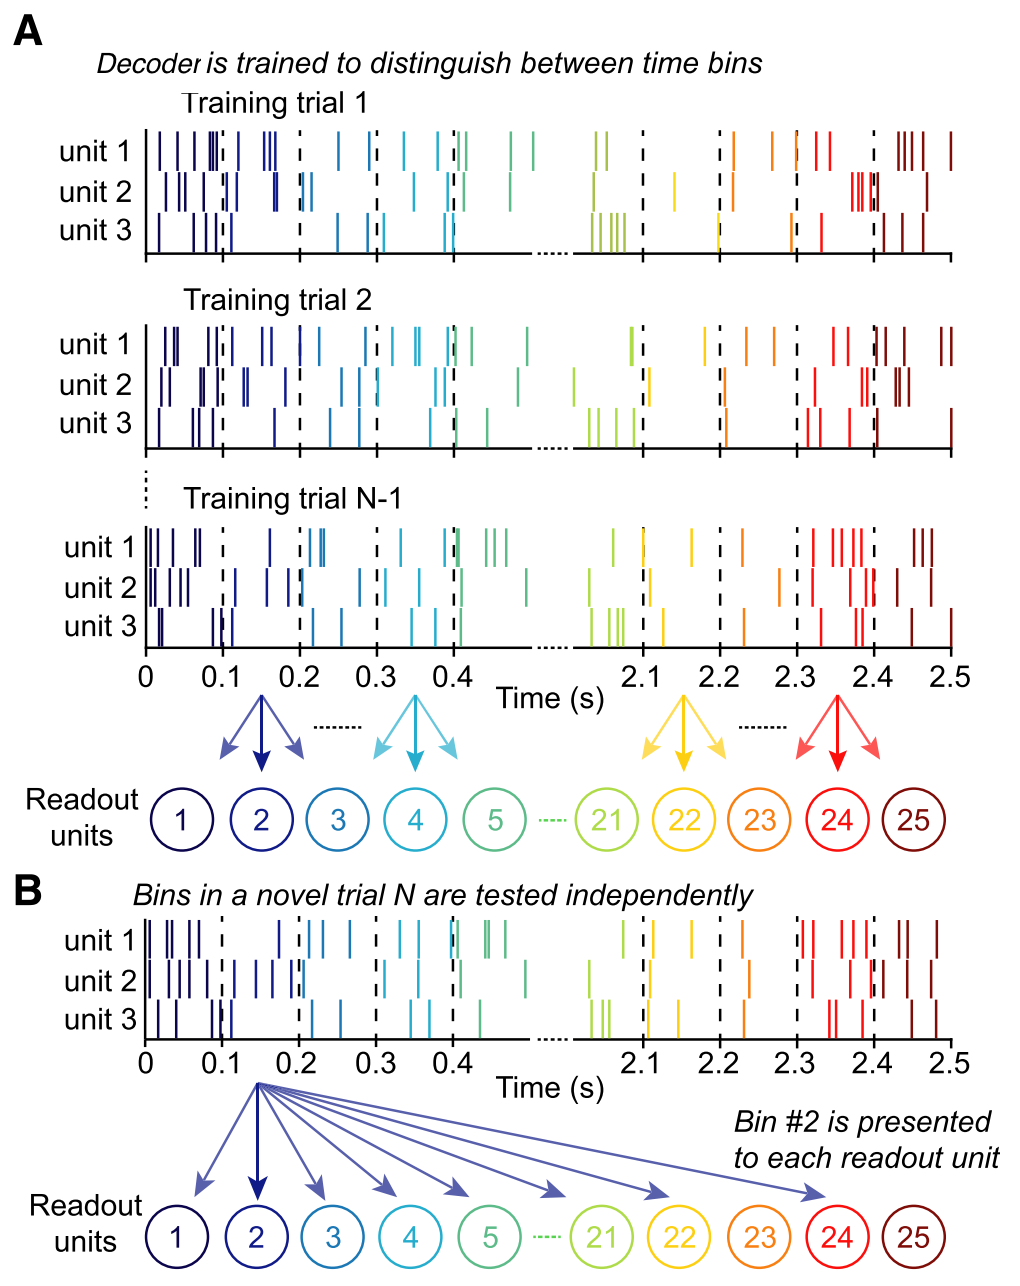
\includegraphics[width=0.83\textwidth]{figures/sketches/decoder.png}
        \caption[Classifier training sketch]{A, Training a classifier. Population activity for simultaneously recorded neurons (only 3 units represented) is transformed into firing rate estimates. The rate estimates are binned into 100 ms time bins. The classifier is trained to distinguish the population activity pattern in each time bin from every other time bin. The output can be illustrated by readouts of the probability per target time bin. B, The  model performance is evaluated using a Monte Carlo cross-validation approach, in which activity patterns from trials not used to train the model is presented to trained models. The example shows bin \#2 of some test trial. Modified from Bakhurin et al. \cite{bakhurin2017differential}}
        \label{fig:decoding}
    \end{figure}

    For each trial, the spike activity within the nosepoke was first transformed in a measure of population firing rate, following the steps described in Subsection \ref{subsec:fr_estimation}. Thereby, we obtained one population firing rate vector in 100~ms time bins, with each neuron corresponding to a vector coordinate. In the case of trials longer than 1.5s, only the first 15 bins were used for decoding analysis. 

    Elapsed time was then decoded from the population firing rates by either classification or regression. Classification requires a population vector to be strictly labeled as only one of the time bins, as illustrated in figure \ref{fig:decoding}. In turn, regression treats the decoding output as a continuous function, and therefore can provide intermediate values within a time bin, such as 450ms or 770ms.

    %Elapsed time was decoded from the population firing rates by either classification or regression. While classification requires a population vector to be labeled as one of the time bins, regression treats the output as a continuous function, and can give values such as 450ms or 770ms.
    Classification was implemented using Linear Discriminant Analysis (LDA) while regression used Bayesian Ridge. While many other algorithms were tested and corresponding hyperparameters tuned, we've chosen to advance our analysis using simpler and untuned algorithms. 

\section{Algorithm comparison}
    In the comparison between possible decoders, to find good hyperparameters for each, we applied a bayesian search using the scikit-optimization library \cite{skopt}. This procedure begins by randomly searching the parameter space, and after some iterations it starts to make estimates of the function values in the parameter space, sampling points with high estimated value. The fit of hyperparameter space is done by gausian processes, and its implementation is dealt with entirely by the library. The length of search was defined for each classifier depending on the number of hyperparameters to tune.
    
    We calculate the value at each point as the mean performance across a 5-fold cross-validation. All the procedure was done using a subset of half the data, selected as every other trial.
    
    We optimized classifiers for the pearson's r metric, and regressors for the explained variance (see section \ref{sec:metrics}).
    
    
    
\section{Bin shuffling}
    
    To test whether the methods used here were statistically significant, we randomized the data to produce ``surrogate'' datasets that, at the same time preserve global statistics and eliminate all causal effects. Applying the same method to the shuffled data, we can establish a baseline for the method and establish the chances of having significant effects by chance, and hence, measure the significance of the effects. The method we used here was the 
    bin shuffling and it was based on methods from \citeauthor{bakhurin2017differential} \cite{bakhurin2017differential}. It was used to break the temporal order of population activity, in such a way as to provide a null hypothesis for the neural activity prediction. To create the shuffled activity, each time bin in a trial was assigned a random activity vector from that trial, without replacement. In the end, each population activity vector is randomly assigned to a time point that does not relate to the original time point where the activity was extracted from.

\section{Performance metrics}
\label{sec:metrics}
    The metrics used for assessing model performance depended only on 1) the final output of the model (prediction) and 2) the correct time (tag). These metrics were given as follows:
    The prediction for all examples is the vector $\hat{y}$, while the correct tag for all the examples is the vector $y$. $N$ is the dimensionality of the vectors. $\bar{x}$ is the sample average of a variable $\sum_{i=1}^N{\frac{x_i}{N}}$. $\sigma$ is the unbiased standard deviation, and $\sigma^2$ is the unbiased variance, $\sigma^2(x) = \sum_{i=1}^N{\frac{(x_i - \bar x)^2}{N - 1}}$.

    % Nome em negrito pode ser suficiente
    \subsection{Explained variance}
        Explained variance provides a quantitative measure of how much the inclusion of the model can account for reducing the data variability. The computation of this measure contrasts the amount of variance in the residuals of the fitted model with the amount of variance in the original data.

        $$ \text{explained variance}(y, \hat{y}) = 1 - \frac{\sigma^2(y - \hat{y})}{\sigma^2(y)}$$
    
    \subsection{Pearson's r}
        Pearson's r is a measure of linear correlation, calculated by normalizing the linear covariance of two variables by their respective variances. 
        
        $$
        \text{Pearson's r}(y, \hat{y}) = 
        \frac{1}{n-1}\frac{\sum{(y - \bar{y})(\hat{y} - \bar{\hat{y}})}}
             {\sigma(y)\sigma{(\hat{y})}}
        $$
    
    \subsection{Modified accuracy}
        We modified the accuracy metric to enable its use in regression. Generally, accuracy is ill-defined for continuous targets, since it has no "similar enough" threshold. Our modified accuracy consists of rounding the continuous output to its closest value before measuring accuracy in its conventional sense. The notation $[\hat{y}]_y$ is the nearest value in $y$ for each value in $\hat{y}$. $\delta(x_1, x_2)$ is the Kronecker's delta, taking the value $1$ when $x_1 = x_2$ and $0$ otherwise. 
        
        $$
        \text{accuracy}(y, \hat{y}) = \frac{1}{N}\sum_{i=1}^{N}{\delta(y_i, [\hat{y}_i]_y)}
        $$
        
        
        
        
        
\chapter{Open Code}
    All authored code is available at https://github.com/EstevaoUyra/spikelearn, under the permissive MIT Licence. All procedures were written in Python, while some wrappers have been written in bash.

% \subsection{Functions and Documentation}
    To enable other researchers to apply the analysis as easier as possible, most of the code was transformed into \textit{functions}. They have been documented using the Numpy style\footnote{Available in https://www.numpy.org/devdocs/docs/howto\_document.html}, which enables automatic generation of documentation web pages via the sphinx package\footnote{http://www.sphinx-doc.org/}. 

% \subsection{Packaging}
    To manage the dependencies, and enable installation of the code, we used the \textit{pip} package manager\footnote{https://pypi.org/project/pip/}. This is done through the creation of a single file called \textit{setup.py}, which contains information about requirements and about the package itself.


\part{Methodological contribution}
\chapter{Data and Processing}
\label{chap:data_processing}

One important factor in our task required consideration before processing the data: The animal had to move in and out of the nosepoke, possibly contaminating the neural activity near the trials with motor activity. We had to make sure that the motor activity would not weight in on the trial activity, and for this end we removed the activity out of the trials before calculating the firing rate. This brought its own challenge, because the firing-rate calculation needed an additional parameter, the padding type, to deal properly with the borders of each trial. In this chapter we compare the results for different values of the parameter.

To obtain firing rates for each recorded neuron, we convolved the spikes with a gaussian (smoothing) and divided them into time bins (binning). In sum, we wanted to go from the PSTH figures (or raster plots) to the firing rates. We can see in figure \ref{fig:padding} that applying a gaussian kernel induces correlations between neighboring time points, in such a way that time points with high spike counts induce medium spike counts in neighbour time points. Without smoothing, the activity in single trials is very sparse (i.e. has few nonzero values), and since the precise spike time of a given neuron may not be so representative of its internal state, this transformation into firing rate may aid the classifier in capturing the information present in the neurons.
    
We can see, specially when averaging trials, how different paddings result in different estimated firing rates at the borders of the window: padding the activity with zeros biases down the average firing rate. In our posterior analysis, except when explicitly stated, smoothing was done with symmetric padding.

\begin{figure}
    \centering
    \begin{tabular}{cc}
    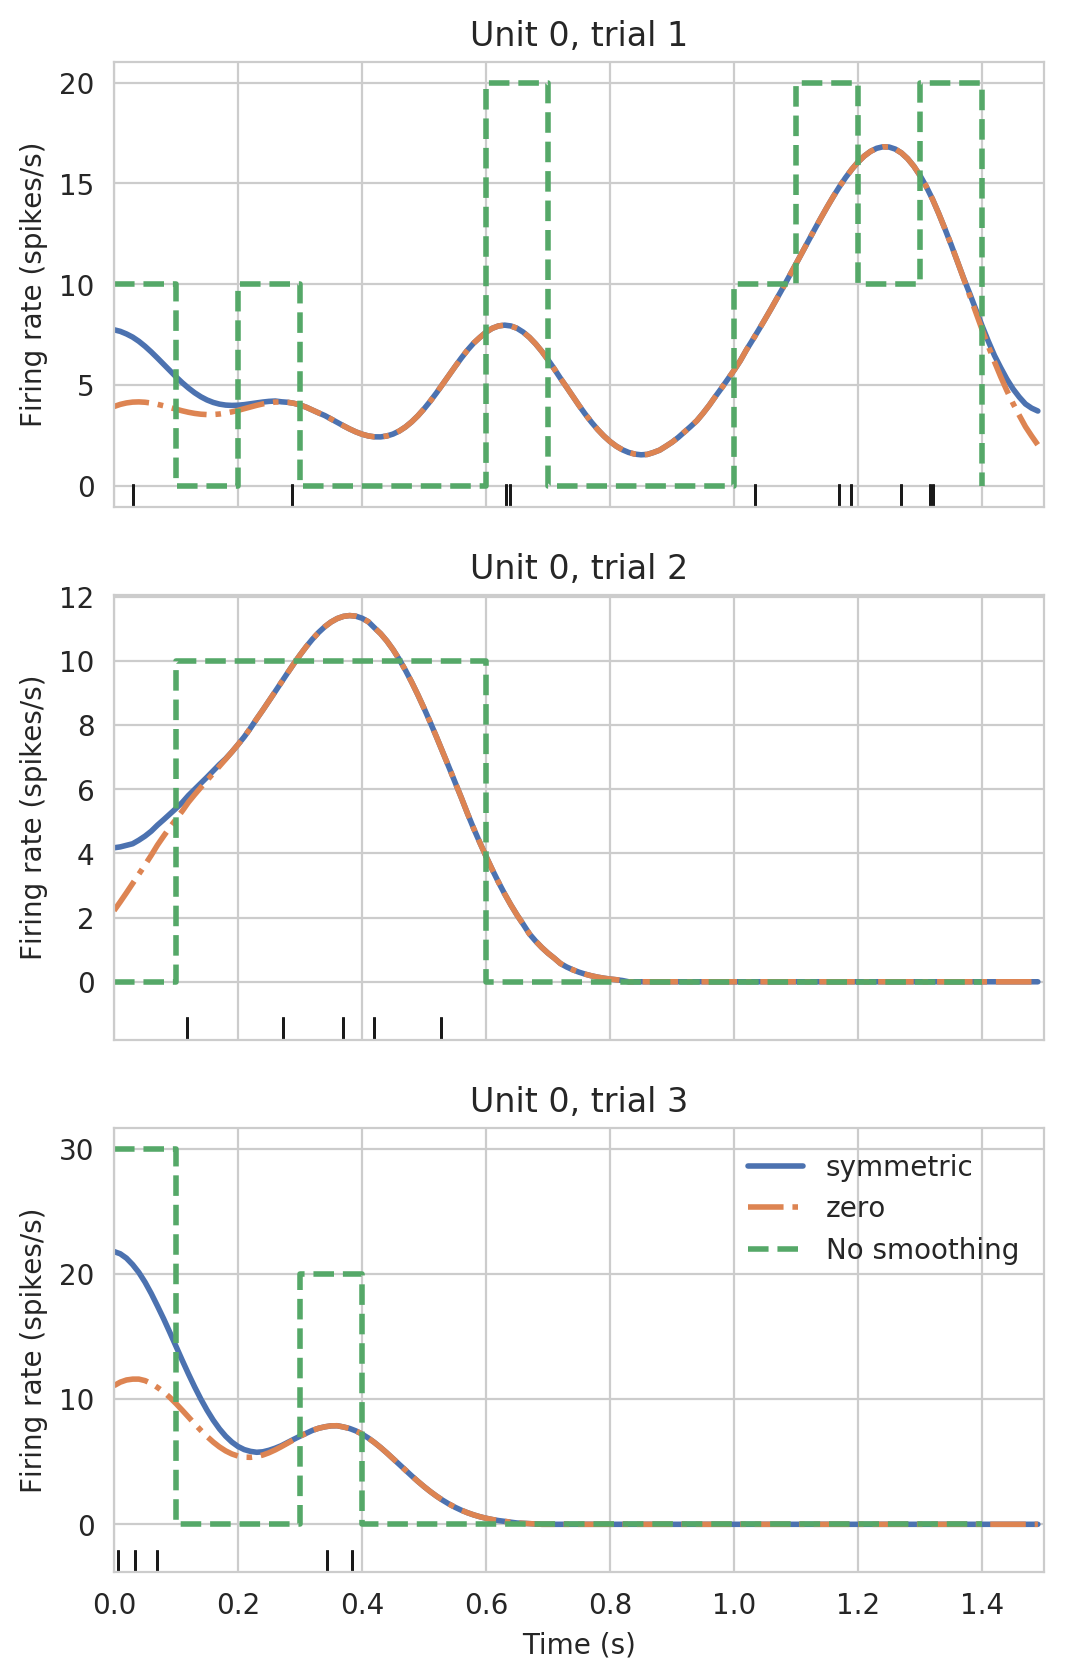
\includegraphics[width=7cm]{figures/one_with_step.png}
    & 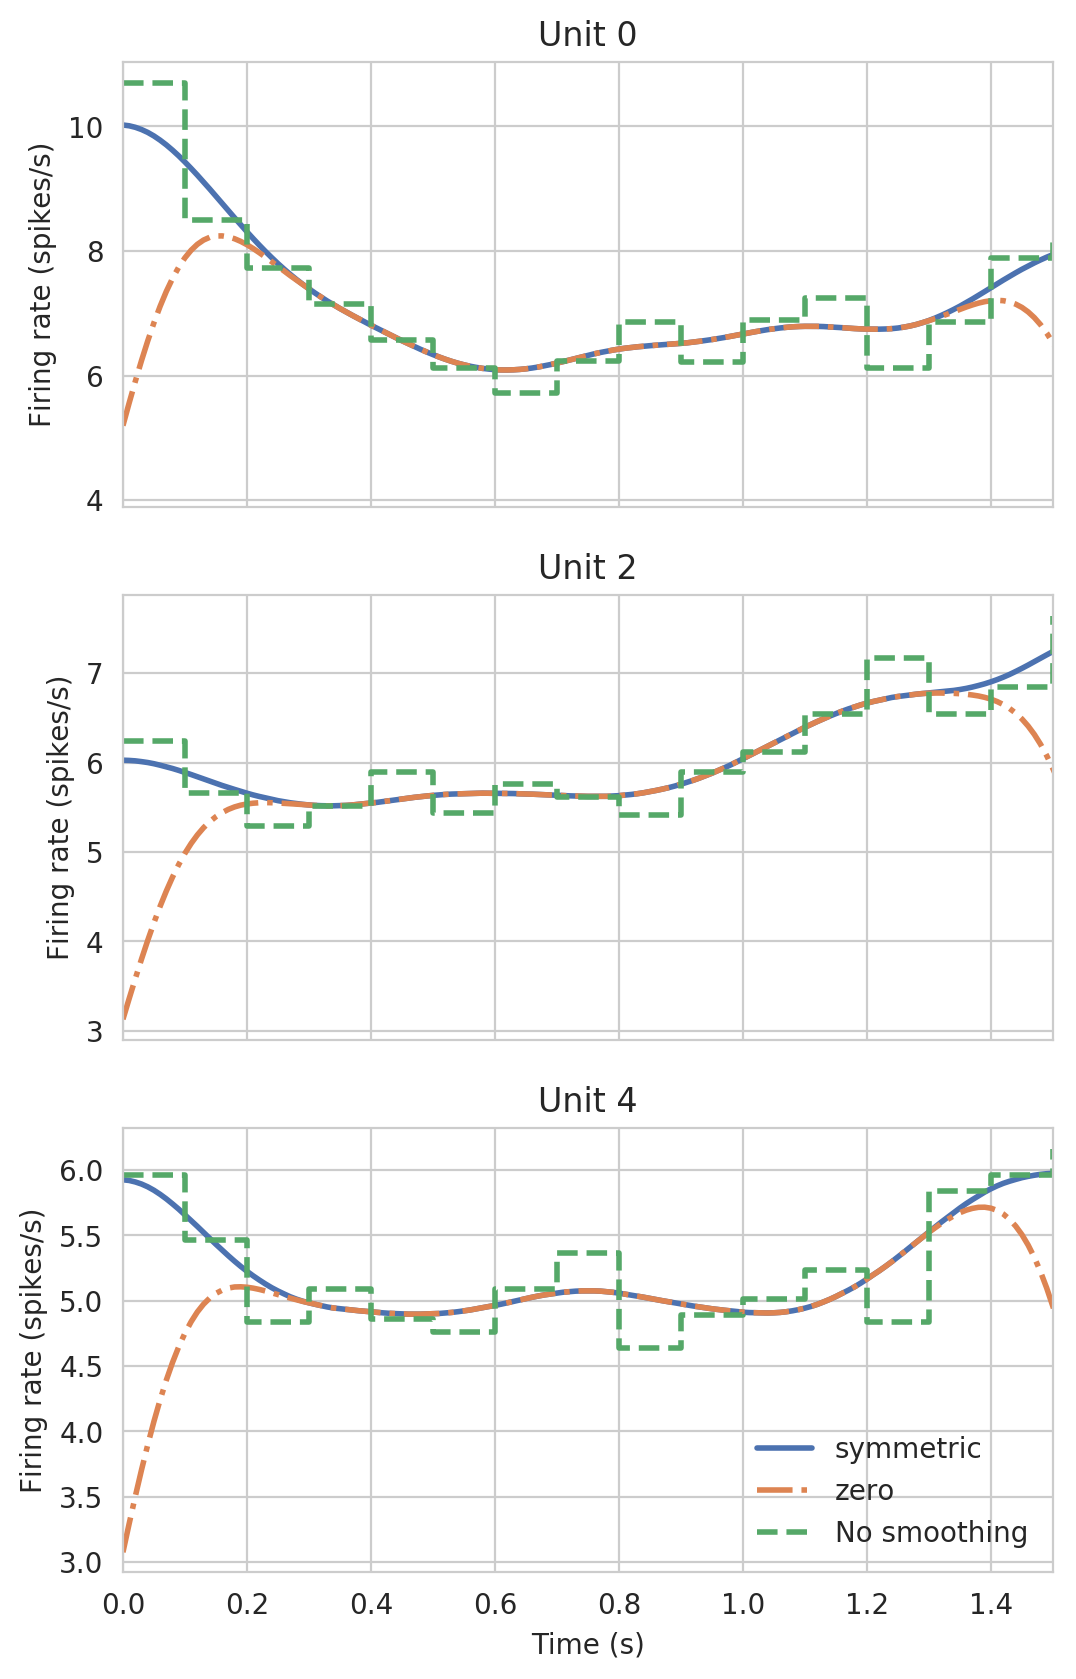
\includegraphics[width=7cm]{figures/mean_with_step.png}
    \end{tabular}
    \caption[Effect of smoothing and padding choices on the estimated firing rate.]{Effect of smoothing the spike counts with a 100ms kernel and padding choices on the estimated firing rate. Left: Single trial firing rates, Right: Mean firing rates. In the left, exact spike times appear as black ticks in the x axis.}
    \label{fig:padding}
\end{figure} 

\begin{figure}
    \centering
    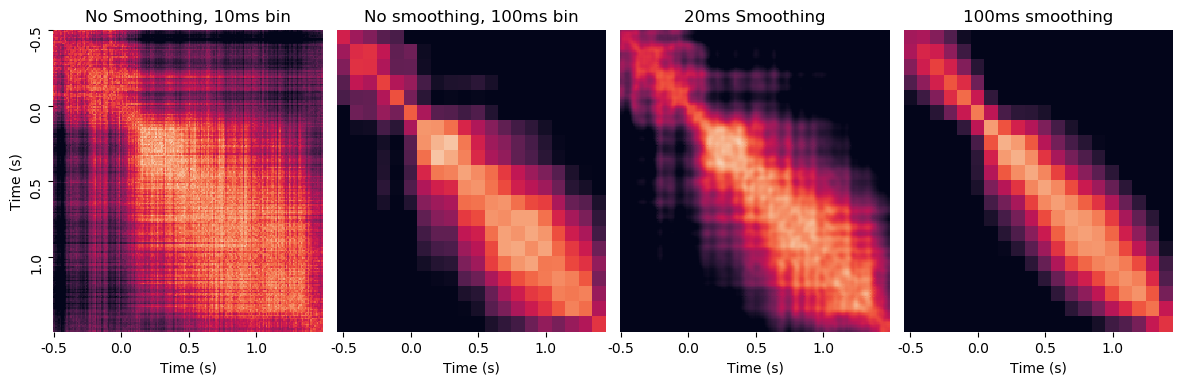
\includegraphics[width=\textwidth]{figures/similarity_comparison.png}
    \caption[Binning and smoothing assessed via similarity matrix]{Binning and smoothing assessed via similarity matrix. Spike count activity at left is binned in small and big time bins, and at the right is smoothed with a narrow and a wide gaussians.}
    \label{fig:mahalanobis_smoothing} 
\end{figure} %No smoothing, bin10 bin100, DRRD10 and DRRD9
    
    % A simple similarity analysis was used in figure \ref{fig:mahalanobis_smoothing} to measure consistency in the dynamics of neural activity. The analysis compares the activity vector of each single time point with the activity vector of another time point, measuring proximity in a space that considers less strongly dimensions in which variability is bigger. We expect to see stronger diagonals when the activity is very similar among trials, indicating that activity vectors coming from the same time point are usually near each other.
    
    % In figure \ref{fig:mahalanobis_smoothing}, we can see at the left that bins that are too small can make it hard to see trial consistencies, in the case of no smoothing, because of the sparsity of spike activity. When we bin in 100ms windows, we can see that activity appears more consistent, what can be also achieved by smoothing with small kernels (e.g. 20ms). A larger kernel (100ms) makes the activity yet more consistent. 
    In all cases, it is clear that the baseline is more similar to itself, and different from the rest of the trial. This is expected since the animal is in a different state, generally approaching the nosepoke, as opposed to standing still with its nose inside. 


\chapter{Regression fits differently than classification}
\label{chap:metrics}

In this chapter we compare how classification and regression differ in the way they fit the data. The results here are focused on the technical distinctions, and not on the theoretical considerations. In chapter \ref{chap:time_is_represented} we show that both methods are able to extract relevant information. The present chapter, alternatively, focuses on bringing about their most explicit distinctions. 


\begin{figure}[ht]
    \centering
    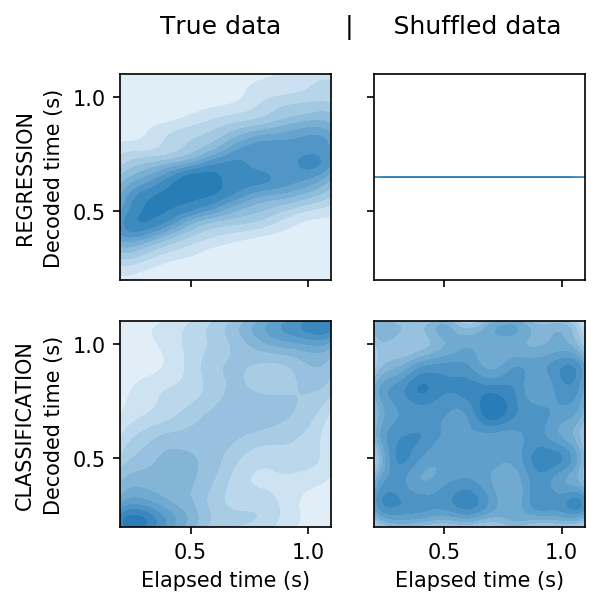
\includegraphics{figures/decoding_kde_bootstrap_vs_true_31.png}
    \caption[Comparison of prediction distributions when data is shuffled]{Comparison of prediction distributions when data is shuffled. Lines refer to the type of algorithm used to assess activity - regression and classification, while columns refer to the type of data - shuffled or not. Darker blues indicate higher density of points. For a given elapsed time, the vertical upon it is the distribution of all predictions calculated over neural activity extracted at that time.}
    \label{fig:decoding_kde_boot}
\end{figure}

To compare our decoding results, we look into the distribution of predictions according to the elapsed time of the activity. We can see the full distribution by kernel-density-estimation in figure \ref{fig:decoding_kde_boot}, and a simpler version with mean and variance in figure \ref{fig:decoding_line_boot}. When decoding shuffled data, the regression cannot find information and always predicts the mean, because this minimizes the expected root squared error. This appears in either plot as a single line located at the mean. Classification has no such strategy, because to the classifier there is no "error size" with respect to the predicted class: predicting a .2 and predicting a .9 are equal-sized errors to an example labeled .3. The mean prediction for each time bin, shown in \ref{fig:decoding_line_boot} is located around in the mean value, and distinguishes from the regression results mainly by the huge error bounds. In figure \ref{fig:decoding_kde_boot}, the prediction randomness caused by shuffling is revealed by the multiple density blobs haphazardly located. By repeating the analysis (not shown here), although the other subplots keep the same appearance, the shuffled classification changes considerably, with the blobs in other locations.

\begin{figure}[ht]
    \centering
    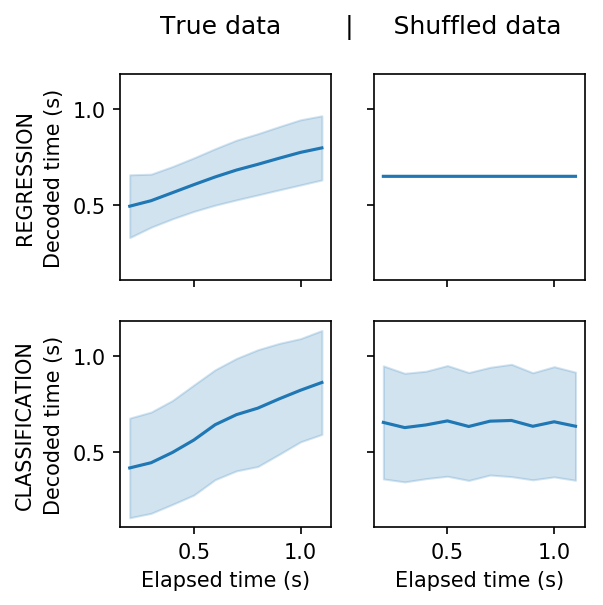
\includegraphics{figures/decoding_line_bootstrap_vs_true_31.png}
    \caption[Summary of prediction distributions comparing when data is shuffled]{Summary of prediction distributions comparing when data is shuffled. Lines refer to the type of algorithm used to assess activity - regression and classification, while columns refer to the type of data - shuffled or not. The darker line is the average decoded value for all data points extracted from a given Elapsed Time. The bands represent the standard deviation around that average.}
    \label{fig:decoding_line_boot}
\end{figure}

With respect to the true data, we can see in \ref{fig:decoding_line_boot} that the mean prediction has a positive inclination, showing that activity from later in the trial is predicted in average with higher values. While this is seen both in classification and regression, they have distinct patterns of errors, showed in \ref{fig:decoding_kde_boot}, with regression tending towards the mean values while classification tends towards the borders. The classification line has a steeper inclination, but also much bigger deviations. 

Classifiers in this task are typically better at predicting the borders of trial (onset and offset), as found in other experiments of our group. This may be an artifact of the number of proximal bins to the one being tested. Specifically, we hypothesize that, because border bins have only one proximal bin -- the previous one for the last bin, and the next one for the first bin -- they are easier to get right. All the other bins in the trial have both previous and next. Regressors, distinctly, having an error measure that is continuous and relates to the distance, do not suffer from the same artifact.

With respect to the metrics we have chosen to compare the models, something very distinct appears as a result of this "strategy" difference. When looking at the Pearson's r between the true labels and predictions, classifiers are comparable to regressors. On the other hand, when we choose to look at the explained variance, we see a huge difference. This is because the classifiers create variance in the residuals when they predict the borders. Regressors, distinct from classifiers, optimize explicitly for the sum of squared errors that gives raise to the residual variance.

\chapter{Algorithm optimization}
\label{chap:results}

We used henceforth classification performance as a proxy to neural representation. Since we want to understand how information about time develops in the brain during learning of the task, we compared this classification performance in the beginning of the session and near the end of the session. Before making this comparison, we tested multiple classifiers to be sure that any kind of information captured by then is not specific to the classifier.
\subsection{Classification}

\section{Rationale}
    \begin{figure}
        \centering
        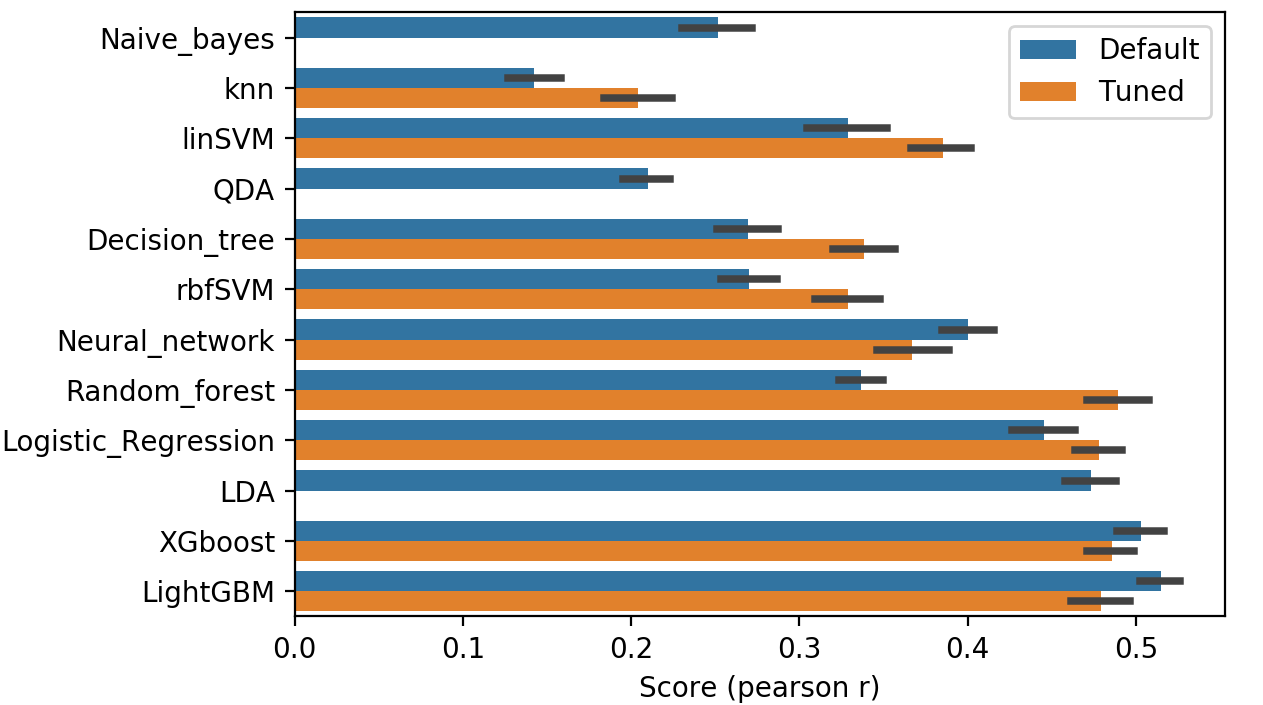
\includegraphics[width=\textwidth]{figures/clf_comparison.png}
        \caption[Comparison of classifiers]{Comparison of classifiers. Default hyperparameters were compared with those resulting from tuning when there were hyperparameters to tune.}
        \label{fig:clf_comparison}
    \end{figure} % Mean performance+-SEM for each classifier tuned and untuned. 
    Firstly, we compared classification performances for different classifiers, in such a way as to make an informed choice for our subsequent analysis. We calculate scores in each tuning step with 5 folds of Monte Carlo cross validation, and evaluate the final scores with 50 folds. Half of the trials were hold out for tuning, trials from the other half were used for evaluation of the final score.
    
    We found big differences in performance between the multiple classifiers tested. Some classifiers have good results out-of-the-box, such as Logistic Regression and Linear Discriminant Analysis (LDA), while some are highly dependent on hyperparameter tuning, such as Random Forest. The results for the gradient boosting classifiers LightGBM and XGBoost are specially interesting, as they have better results on the default configurations than after tuning, which is probably due to the fact that we were tuning 10 different hyperparameters, making us prone to overfitting the tuning.
    
    \begin{figure}
        \centering
        % \includegraphics[width=\textwidth]{figuras/methods/learning_curves_sppfc.png}
        \caption{Classifier learning curves}
        \label{fig:clf_curves}
    \end{figure}
    % Colocar aqui somente para os melhores. Colocar os outros no material suplementar.
    For most classifiers, there is significant decoding for as little as 10 trials in the training set. As expected, the classifier's performance increases with the number of trials used for training it. It is even possible that a bigger training set would give us even higher scores, pointing to the importance of having big experimental sessions with many trials. Hence, if we want to compare the information contained in the neural activity in different moments in a session, we have to ensure their classification models are trained with the same number of trials.



\part{Contribution}
\chapter{Animals Learn fast}
\label{chap:learning}

% Recent findings from our group suggest that animals can learn the DRRD in a single 50-minute session \cite{ReyesDRRD}. We designed our methodology based on that expectation. Hence, we compared the distribution of the response duration in different stages of the session 

We designed our methodology based on the expectation that rats learn the DRRD task in a single session, as previous findings from our group showed~\cite{ReyesDRRD}. To verify whether this assumption holds to our data, we compared the distribution of response duration in different stages within each session. However, to make sure rats were engaged in the task, aiming to receive rewards as frequently as possible, we analyzed the duration of periods between trials (intertrial intervals, ITI). We hypothesized that those intervals indicate the level of engagement of rats while performing the task -- more extended periods between nose pokes indicate lack of interest in reward and less engagement in the task.

As described in the session \ref{sec:acquisition}, we analyzed two distinct data sets, one in which the animals trained for several hours and the other in which they trained for fewer hours but with more than one day of training.  Hence we gathered data differently for these two groups of animals. The average number of trials in the long sessions was $1149 \pm 384$ trials and provided about $660 \pm 260$ correct trials. In turn, in short sessions consisted in $570 \pm 181$ trials and with a smaller amount of correct trials ($284\pm 100$) -- about half the number obtained in long sessions. Thus, for group 1, of animals which performed a single long session (rats 7, 8, 9 and 10), we split each session into its first and second half. In turn, for group 2, of animals which performed two shorter sessions (rats 3, 4, 5 and 6), we analyzed the first and second session separately. This procedure thus leads to proportional sets of trials divided into earlier and later parts for each animal.

%Our methodology is centered on the expectation that learning our task occurs as fast as in a single session. To confirm this expectation we compare the distribution of responses across learning stages. Specifically, we divide the session into the first and second half for the group with long sessions, and into the first and second sessions for the group with short sessions. This is because for the first group we had long sessions of more than 1000 trials $(1149 \pm 384)$ with sufficient correct trials $(660 \pm 260)$. For the second group of animals, in which sessions were half as long (with $570 \pm 181$ trials), there were only and $284\pm 100$ correct trials, less than half compared to the first group. This comparison is preceded, however, by an assessment of the engagement of rats: we want to assure that animals intend to obtain reward as frequently as possible.

\section{Rats disengage in long sessions}
    A central assumption of our study is that animals maximize the amount of reward received, as assumed in conditioning studies in general. In our task, animals have to stay in the nosepoke long enough to receive their reward but holding too long delays the reward. When animals seek reward as fast as possible, we expect that they to remain in the nosepoke as little as possible to receive the reward. In this case, increases in response durations can be attributed to learning of the underlying time interval. Moreover, because the animals can start new trials whenever they want, we expect them to do so with little delay. Alternative reasons for increased response times could be diminished interest in the reward, satiety or tiredness. We hypothesized that, if the animal disengages the task, the interval between trials (ITI) should also increase.

    \begin{figure}[h]
        \centering
        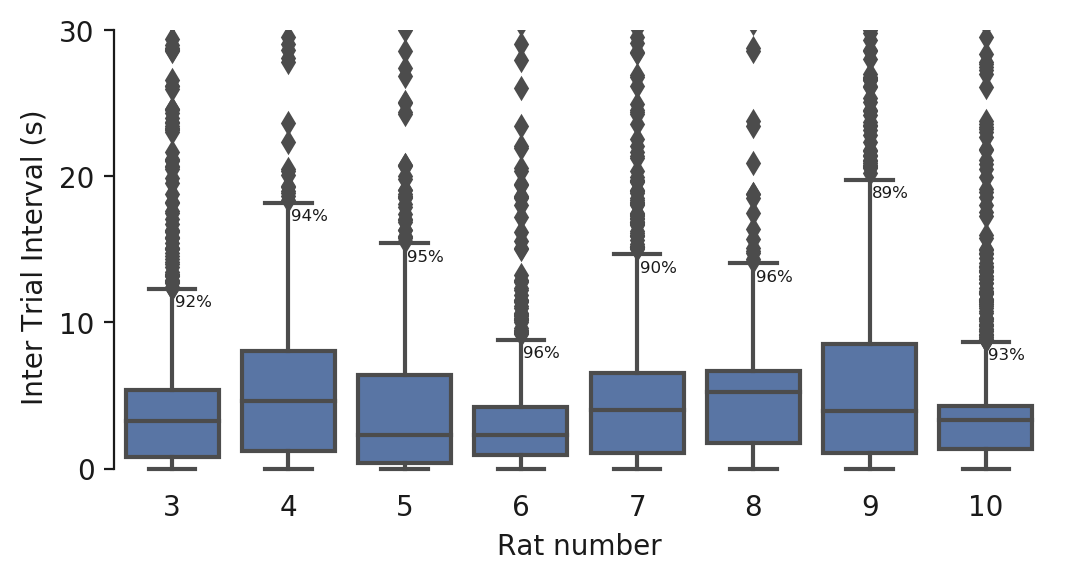
\includegraphics[width=\textwidth]{figures/inter_trial_boxplot.png}
        \caption[Time between trials is in the order of seconds]{Time intervals between trials are in the order of seconds. The distribution of all inter-trial intervals for each rat in boxplot quantiles. The horizontal trace above each box shows the last point up to 1.5 IQRs (Inter Quartile Ranges) of the .75 quartile, a common threshold to define outliers. The percentage right below that line shows how many of the points are below the threshold.}
        \label{fig:iti_box}
    \end{figure}
    
    In figure \ref{fig:iti_box} we can see that most of the intervals are below 20 seconds. Specially in rats 6 and 10, more than 90\% of ITIs were under 10 seconds. Although there is variation, intervals are in the order of low tens of seconds, and thus seem to be consistent with reward seeking. On the other hand, there are many outliers: whereas figure \ref{fig:iti_box} showed up to 30s, there are some intervals with more than 10 minutes between trials. If these large intervals were distributed all along the session, this could complicate our findings. However, if they are concentrated later in the sessions, they may be indicative of natural tiredness or satiety of a previously engaged animal.
    
    \begin{figure}[ht!]
        \centering
        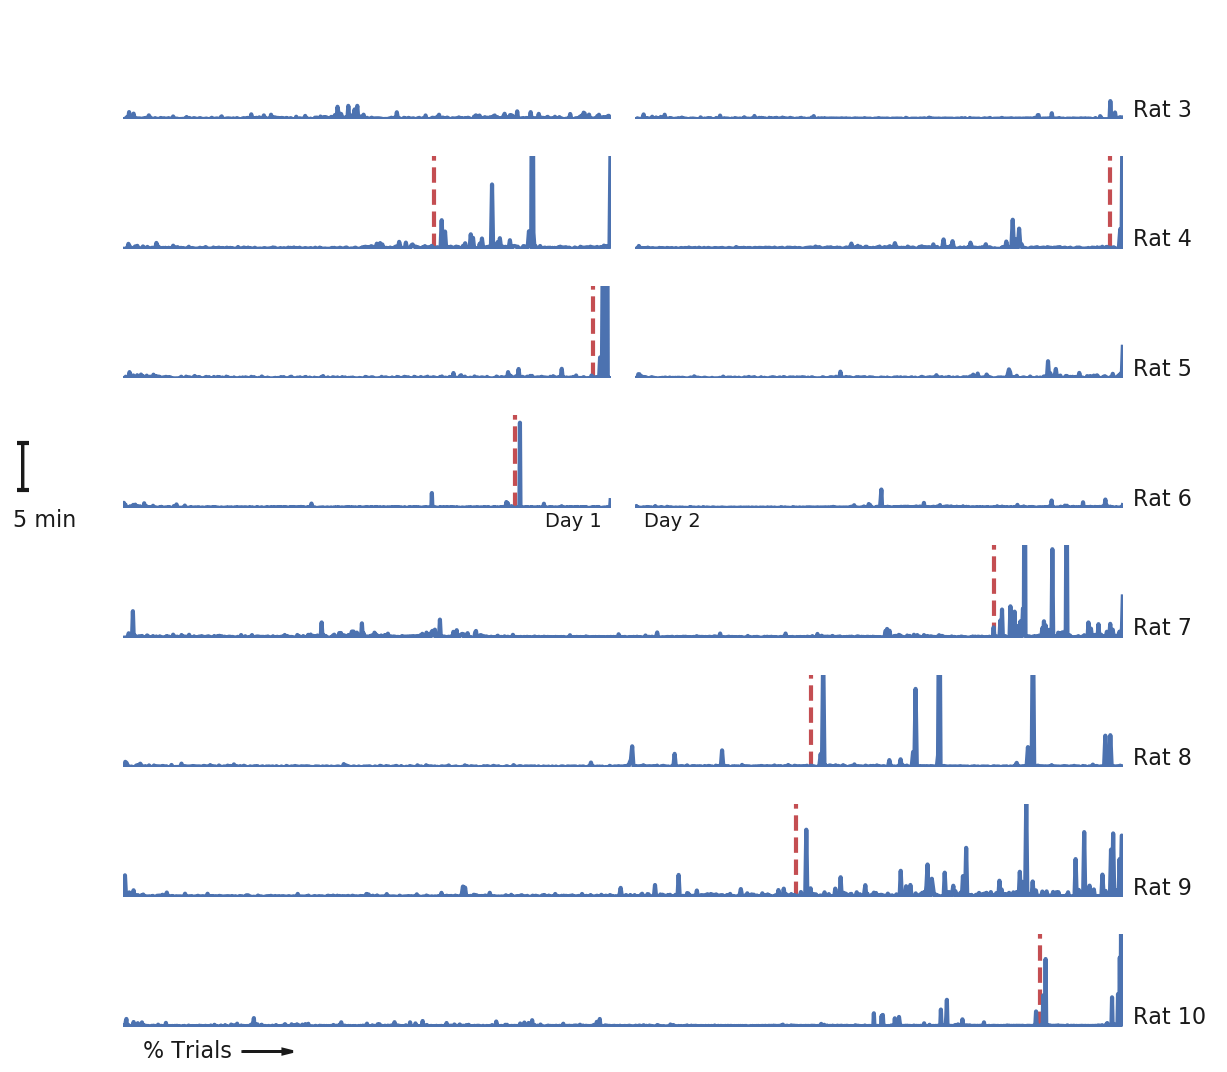
\includegraphics[width=\textwidth]{figures/inter_trial_alongtrial.png}
        \caption[Rats disengage in long sessions]{Rats disengage in long sessions, increasing their resting period between trials, waiting for minutes without engaging in the nosepoke. Each row shows the ITI of a single animal, ordered by trial, and normalized by the session duration. The upper four rows correspond to animals in the group 2, with two shorter sessions, and two respective columns. The red demarcation displays the limit of engagement, measured as the first sum of 5 or more minutes ITI in 5 consecutive trials. Posterior trials have been removed from subsequent analysis,}
        \label{fig:iti}
    \end{figure}
    
    
    To understand better how this long outlier ITIs are distributed along the session, we plotted the ITIs of each trial in sequence, in figure \ref{fig:iti}. The figure shows the two shorter sessions of animals from the group 2, and the single long session from group one. We can see that indeed the ITIs increase later in the session for almost all recorded sessions, including some of the shorter. There is some heterogeneity in the disengagement patterns: In rat 9, many medium ITIs of 1 to 5 minutes can be seen close together, with a single bigger peak. In rat 8 there are less medium ITIs, and some peaks of 10 or more minutes are separated by small ITIs (< 1 min). In rat 5, a single big peak is surrounded by small ITIs.
    
    Disregarding the heterogeneity in ITI increase, longer ITIs are more frequent later in the session, supporting the hypothesis that animals get tired (or satiated) and disengage the task after some time. We defined a threshold for rejecting trials after a ``disengagement point'' in a reproducible manner. For such, we calculated the sum of ITIs for each 5 consecutive trials, and excluded all trials after the first sum above 5 minutes. This could be reached by a single trial with ITI bigger than 5 minutes, by five consecutive trials with 1 min of ITI each, by one ITI of 3 minutes followed by another one of 2 minutes, and so on. Figure \ref{fig:iti} shows the point at which sessions were pruned according to this criterion (red dashed line).
    
\section{Learning progression is diverse}
    \begin{figure}[ht!]
        \centering
        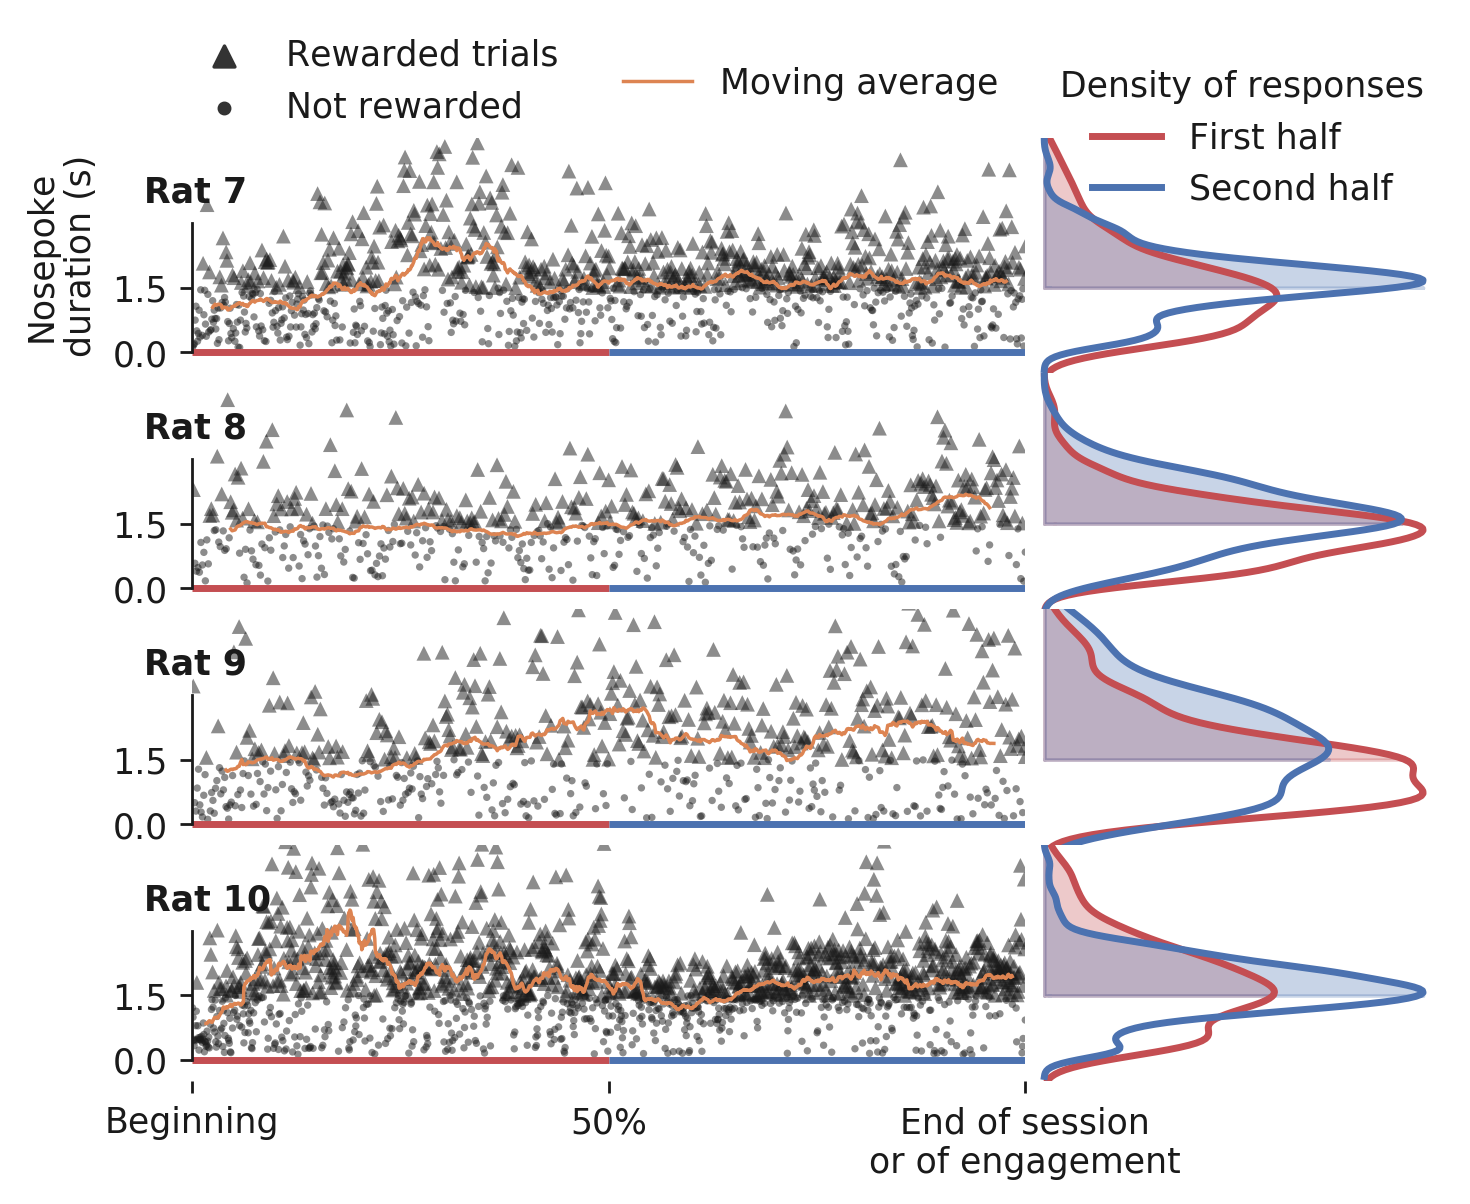
\includegraphics[width=\textwidth]{figures/behavior_group_1_with_avg_bold.png}
        \caption[Behavior across single session]{Behavior across single session, for four subjects. The circles and triangles represent the incorrect (shorter than 1.5s) and correct trials (longer than 1.5s) respectively. An orange line represents the moving average of 50 consecutive trials. The density plot on the right shows the distribution of responses in the first and second halves of the session. Rewarded trials are shaded, in such a way that the increase in rewarded trials is proportional to the difference in blue minus red shadings.}
        \label{fig:behavior}
    \end{figure} 
    
    \begin{figure}[ht!]
        \centering
        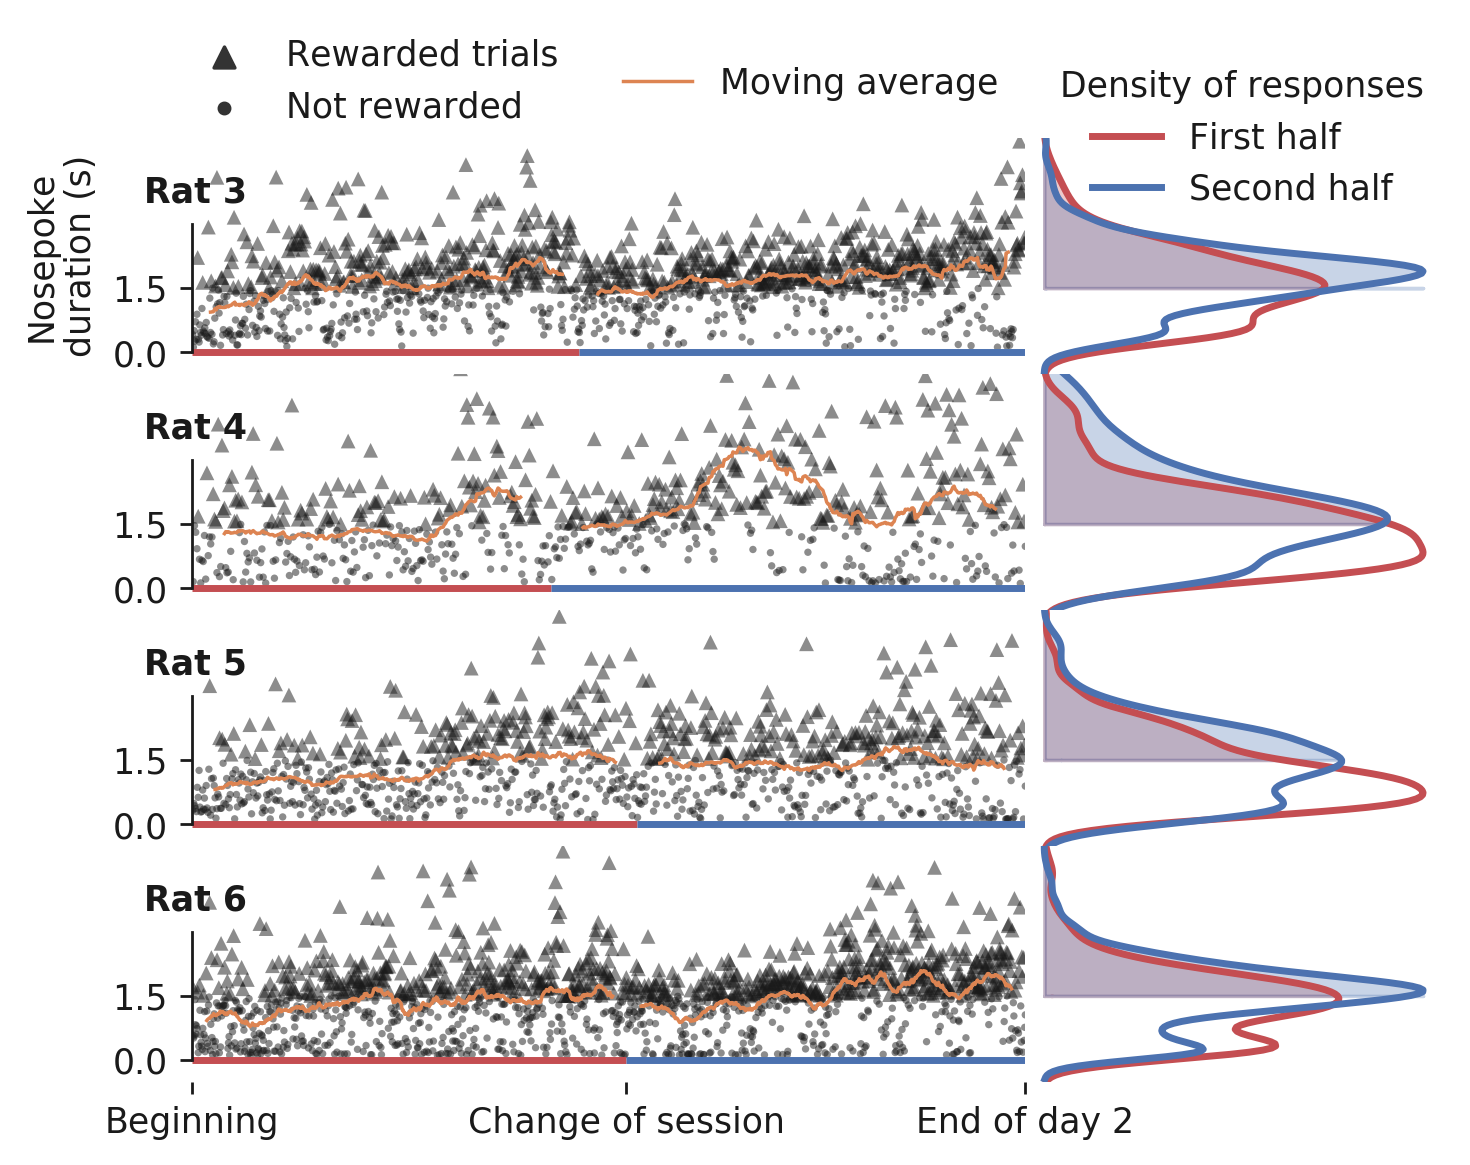
\includegraphics[width=\textwidth]{figures/behavior_group_2_with_avg_bold.png}
        \caption[Behavior across two sessions]{Behavior across two shorter sessions, for four subjects. The circles and triangles represent the incorrect (shorter than 1.5s) and correct trials (longer than 1.5s) respectively. An orange line represents the moving average of 50 consecutive trials. The density plot on the right shows the distribution of responses in the first and second sessions. Rewarded trials are shaded, in such a way that the increase in rewarded trials is proportional to the difference in blue minus red shadings.}
        \label{fig:behavior2}
    \end{figure}
    
    We show the responses for each group of animals in figures \ref{fig:behavior} and \ref{fig:behavior2}. The responses are highly variable, from milliseconds to seconds, in such a way that there are rewarded trials even early in the beginning of the session. In some animals the variability in response duration decreases perceptively (e.g. 7 and 10) and in one of them it increases (i.e. 9). This can be best seen in the density plots, showing distribution of responses in the first and second half.
    
    The moving average drifts up and down, in some rats more than in others. There are rats in which the drift is closer to monotonic. In them, variation between near trials seems smaller, for example rats 6, 8 and 9. Specially in rat 8, the moving average changes smoothly, contrasting with rats 4, 7, and 10, whose moving average has peaks early on and descends afterwards. Rat 10 reaches a moving average duration double the criterion in the first half of the session, with huge variance in its responses, before reducing the duration and variance, and centering responses around the criterion of 1.5 seconds.

\section{Rewarded responses show learning in few hundred trials}

    Looking at figures \ref{fig:behavior} and \ref{fig:behavior2}, we can see that the proportion of rewarded trials increases with training. The proportion is just the count of rewarded trials over the total number of trials. Rewarded trials are those with duration bigger than the criterion of 1.5s, and can be seen in the upper part of each behavior plot. The upper part of the density plots, above the dashed line, indicates this proportion in the area under each curve. We tested the significance of this increase separately for each group using paired-sample t-tests, and found that both are significant. This was calculated as follows: For group 1, we compared the ratio of reinforced trials in the first versus second half of the session, evaluating to p = 0.037 (T=3.564). For group 2, the first session was compared with the second, evaluating to p = 0.0002 (T=20.756). In either case, all trials after the point of no-engagement were excluded before calculation of the ratio of reinforcement.
    
    In sum, although the precise progression of response times is different for each animal, they all increase their rate of correct responses. We compared here two distinct learning stages, showing animals indeed learn and change their behavior really fast. The same learning stages will be compared with respect to their neural activity and time representation in chapter \ref{chap:rep_changes}
    
\chapter{Time is represented in the neural activity}
\label{chap:time_is_represented}

Here we measured whether there is a representation for time in neural activity, based on single-unit recordings on rats' Pre Frontal Cortex. For such, we compared decoding performance in the original data versus in bootstrapped data, which is created by shuffling the time bins of the original data in each trial. The fundamental distinction between shuffled data and the original is that the temporal order has been disrupted. If decoding performance on shuffled data is equal to the original, then we can infer that the temporal ordering of activity is not essential for decoding, and consequently it is not time that is being decoded. Alternatively, if decoding performance is significantly better in the original activity, then time-ordering is driving decoding performance. 

The neural population activity is averaged in bins of 100ms each, from the nosepoke onset (0 - 100 ms) until 1500ms, for a total of 15 population activity vectors per trial. Each bin is tagged with its starting time. In classification the tag is treated as a label, and the problem is treated as multiclass classification: each population vector is classified as one of the 15 possible labels (0, 100, 200, ..., 1400). Alternatively, in regression the tag is treated as a continuous variable, and population vectors are mapped to real values, that can be intermediate values between the bins (e.g. 150). Moreover, in both cases we measure the performance using the explained variance (see \ref{sub:expvar})

\section{We can predict elapsed time using the instantaneous firing rate}
    \begin{figure}
        \centering
        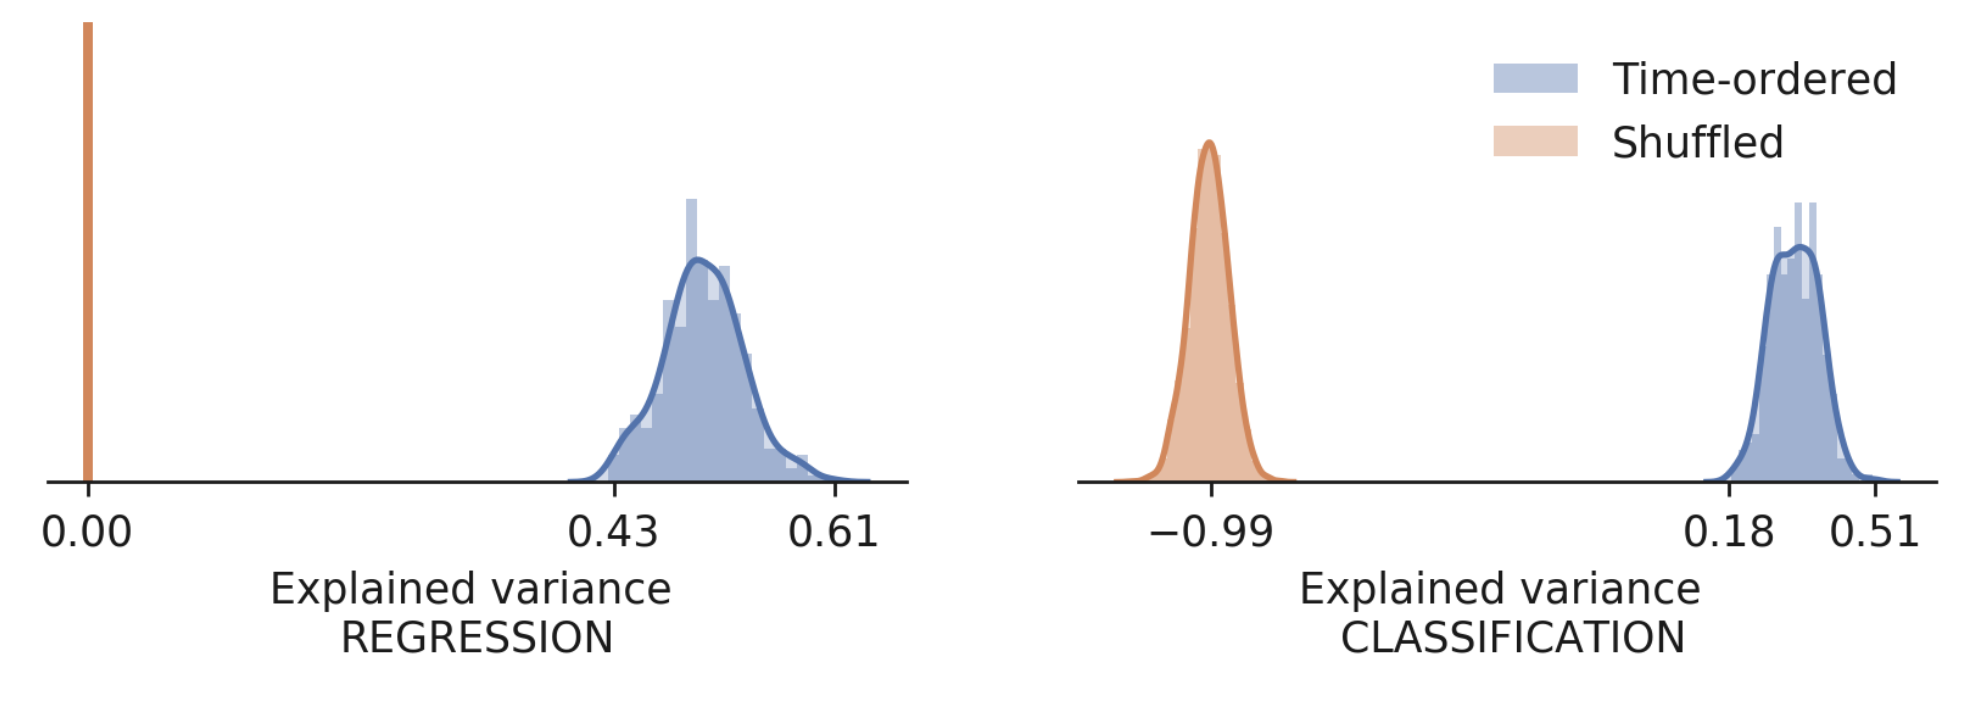
\includegraphics[width=\textwidth]{figures/bootstrap_distribution.png}
        \caption[Comparison between classifier predictions for time-ordered versus time-shuffled population activity]{Comparison between classifier predictions for time-ordered versus time-shuffled population activity. The figure shows the distribution of decoding performances for two decoding methods, in each case comparing with performance in the time-shuffled activity. Either using classification or regression, the population activity differs considerably from the bootstrap, having no overlap.}
        \label{fig:bootstrap_distribution}
    \end{figure}
    
    In figure \ref{fig:bootstrap_distribution} we compare the distribution of decoding performance between shuffled and time-ordered population activities. The distributions are completely separated, giving a p-value of approximately 0 (T-values 974 and 486 for regression and classification) in a t-test. The divergence from bootstrapped data is robust to whether we use regression or classification, as in both cases the distributions have no overlap. The choice of metric also does not change results, in the cases of Pearson's r and accuracy (not shown). 
    
    \begin{figure}[ht]
        \centering
        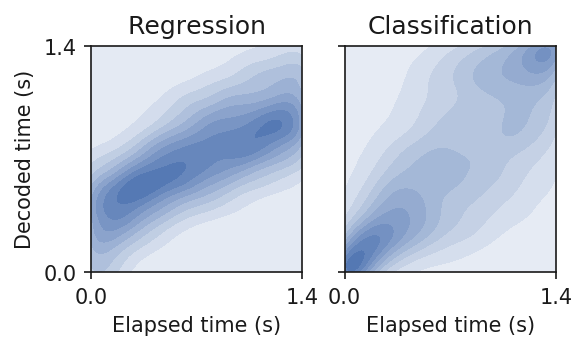
\includegraphics{figures/clf_reg_kde_simple.png}
        \caption[Distribution of predictions show structure]{Distribution of predictions show structure. Figures show two types of algorithm used to assess activity - regression and classification. Darker blues indicate higher density of points. For a given elapsed time, the vertical upon it is the distribution of all predictions calculated over neural activity extracted at that time.}
        \label{fig:decoding_kde_boot}
    \end{figure}
    
    To further assess our decoding results, we look into the distribution of predictions according to the elapsed time of the activity. To this end, we follow a k-fold cross-prediction approach: we separate the trials into 20 groups, or \textit{folds}, evaluating predictions for each fold after training in the 19 other folds. The folds are approximately the same size, with each trial giving rise to 15 predictions, one for each bin of population activity.
    
    We can see the full distribution by kernel-density-estimation in figure \ref{fig:decoding_kde_boot}, and a simpler version with mean and variance in figure \ref{fig:decoding_line_boot}. We can see in \ref{fig:decoding_line_boot} that the mean prediction has a positive inclination, showing that activity from later in the trial is predicted in average with higher values. While this is seen both in classification and regression, they have distinct patterns of errors, showed in \ref{fig:decoding_kde_boot}, with regression tending towards the mean values while classification tends towards the borders. Anyhow, the positive inclination is indicative of the presence of information in the neural activity, and is consistent with the positive evaluation of metrics shown in \ref{fig:bootstrap_distribution}.
    
    \begin{figure}[ht]
        \centering
        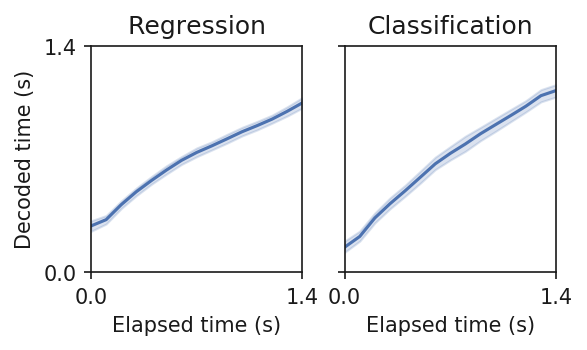
\includegraphics{figures/clf_reg_mean_simple.png}
        \caption[Summary of prediction distributions have positive inclination]{Summary of prediction distributions have positive inclination. Figures show two types of algorithm used to assess activity - regression and classification. The darker line is the average decoded value for all data points extracted from a given Elapsed Time. The bands represent the standard deviation around that average. Since the distributions are not necessarily gaussian, as can be seen in figure \ref{fig:decoding_kde_boot}, the mean and standard deviation are not a full description. Nevertheless, the positive inclination shows there is a tendency to decode bigger times for neural activity coming from bigger elapsed times in the trial.}
        \label{fig:decoding_line_boot}
    \end{figure}

% \section{There is time-warping consistent with timing behavior}



\chapter{Time representation changes with learning}
\label{chap:rep_changes}

To measure how the time representation changes with learning, we compared the neural activity extracted from distinct learning stages, separating each group in the same way as described in chapter \ref{chap:learning}. Specifically, we divide into the first and second half of the session for the group with long sessions, and into the first and second sessions for the group with short sessions, and analyze each separately. 

We have measured the quality of time representation using the same machine learning regression technique from the previous chapter. The number of neurons used in each group and each area was the same, and was kept constant in the multiple learning stages. This was accomplished by sampling a subset of neurons for each area/day. Because one of the merged datasets had only 46 neurons, we selected 46 random neurons for training each model as a pre-processing step. Moreover, models have been trained using the same number of trials, selected once at the beginning of the analysis.

For each neuron pool we repeated the analysis 100 times, measuring the performance metrics for each single run. To calculate the distribution of predictions, we used the same cross-prediction analysis explained in chapter \ref{chap:time_is_represented}. 

\section{Striatum enhances its representation while mPFC decreases}

    \begin{figure}[ht]
        \centering
        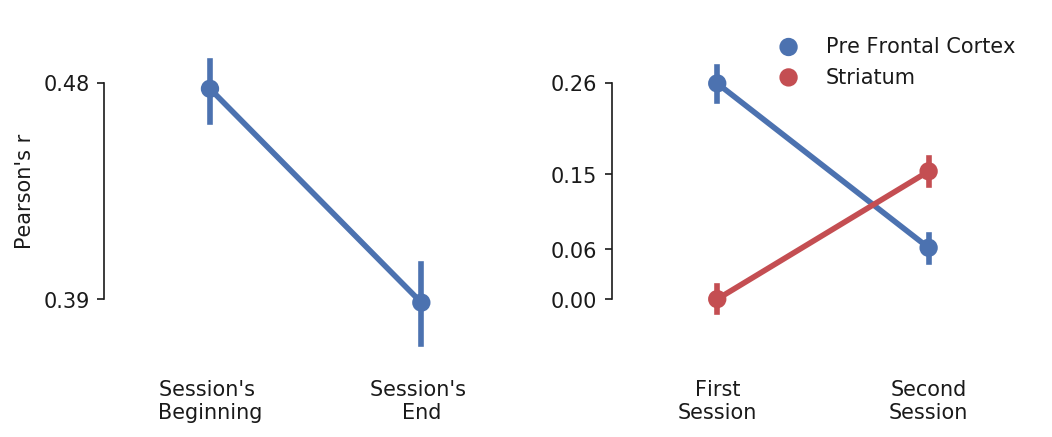
\includegraphics[width=\textwidth]{figures/pearson_comparison_before_after_learning.png}
        \caption[Comparison of classifier performances in distinct learning stages, by Pearson Correlation]{Comparison of classifier performances in distinct learning stages, by Pearson Correlation. Left: Group 1 at first half vs second half of session. Right: Group 2, in the first vs the second smaller sessions. In the vertical, we show the performance of the classifier as measured by Pearson's r. Values shown in the vertical axes correspond to the mean values of data points, shown as circles. The analysis was repeated 100 times, and error bars correspond to the confidence intervals of 95\% calculated by 1000 bootstrap averages of 100 samples with replacement.}
        \label{fig:evolution_representation_pearson}
    \end{figure}

    \begin{figure}[ht]
        \centering
        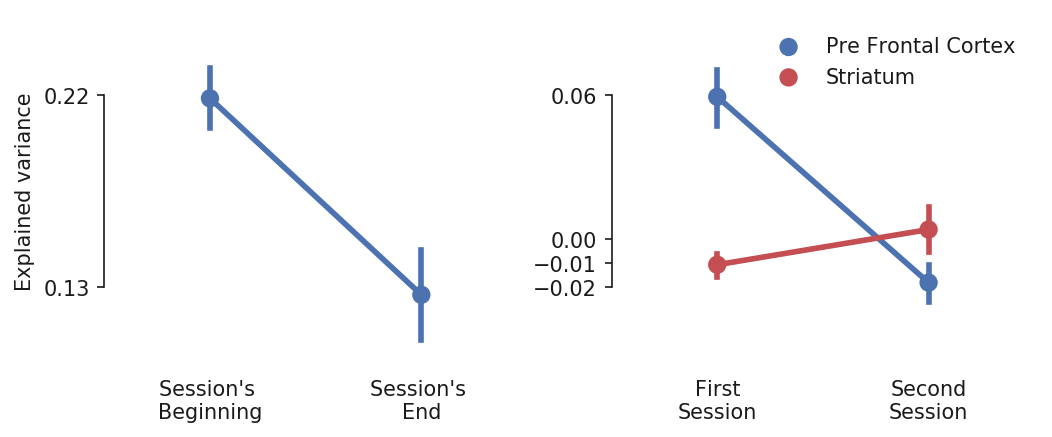
\includegraphics[width=\textwidth]{figures/expvar_comparison_before_after_learning.png}
        \caption[Comparison of classifier performances in distinct learning stages, by Explained variance]{Comparison of classifier performances in distinct learning stages, by Explained variance. Left: Group 1 at first half vs second half of session. Right: Group 2, in the first vs the second smaller sessions. In the vertical, we show the performance of the classifier as measured by Pearson's r. Values shown in the vertical axes correspond to the mean values of data points, shown as circles. The analysis was repeated 100 times, and error bars correspond to the confidence intervals of 95\% calculated by 1000 bootstrap averages of 100 samples with replacement.}
        \label{fig:evolution_representation_variance}
    \end{figure}

    
    When we compare the performance of classifiers as measured by Pearson correlation (figure \ref{fig:evolution_representation_pearson}), we see opposite trends for the two recorded areas. Performance in the mPFC decreases in both groups, while in the second group performance in the Striatum increases. The same pattern can be found in \ref{fig:evolution_representation_variance}, when measuring the same results with the explained variance metric. The main distinction between the results from each metric resides in the second session of the striatum, that is closer in value to the second session for the mPFC. All the distinctions between learning stages are statistically significant, shown in table \ref{tab:statistics_learning_stage}. 
    
    In terms of Pearson's r, the only data in which the regression had null performance was the first session of the Striatum, in \ref{fig:evolution_representation_pearson}. If we look at the prediction distribution in \ref{fig:kde_comparison_days}, it is possible to see that the predictions are very close to a horizontal line, similar to the shuffled data. Differently, in the second session the distribution shows positive inclination, consistent with the increase in Pearson's r score.

    \begin{figure}[ht]
        \centering
        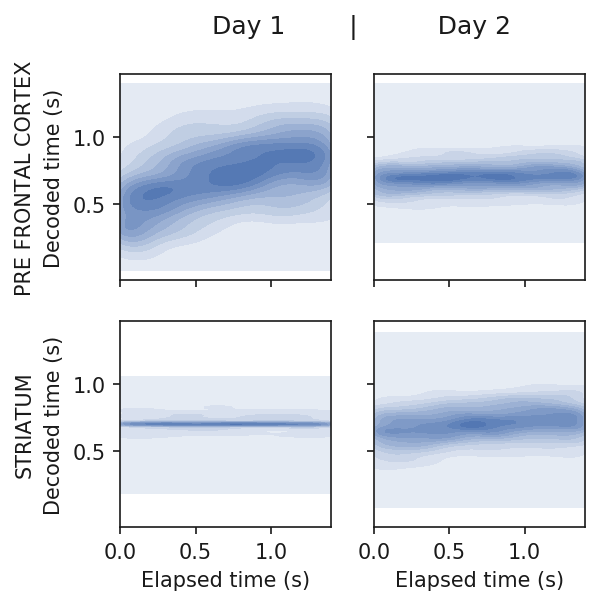
\includegraphics{figures/single_regression_results_comparing_days.png}
        \caption[Distribution of predictions changes with learning]{Distribution of predictions changes with learning. Figures show regression predictions in two areas and two days. The rows correspond to the area being tested, and the column to the day. Darker blues indicate higher density of points. For a given elapsed time, the vertical upon it is the distribution of all predictions calculated over neural activity extracted at that time. The main diagonal shows more inclination in the distributions, while the secondary diagonal is closer to a flat line.}
        \label{fig:kde_comparison_days}
    \end{figure}
    
    The increase in decoding performance for the striatum is accompanied by a decrease in decoding performance for the medial Pre Frontal Cortex. This is found in both groups of animals, as shown in the negative slopes of blue lines in figure \ref{fig:evolution_representation_pearson}. In the prediction distributions of figure \ref{fig:kde_comparison_days}, we can see that in day 2 the distribution of predictions decreases in variance. The distribution of day 2 if much closer to a horizontal line in the mean predicted value, with less of the positive inclination that is indicative of correct performance.
    
    % The explained variance was null or negative in both sessions for the striatum
    
    % Medial Pre Frontal Cortex decreased its inclination
    
    \begin{table}[ht]
        \centering
        \begin{tabular}{l|c|c|c}
            \hline
            Subjects & \multicolumn{1}{l}{Group 1} & \multicolumn{2}{l}{Group 2}\\
            Area & mPFC & mPFC & Striatum \\
            \hline
            Pearson's r         & $-8.19 \quad 10^{-12}$ 
                                & $-14.50 \quad 10^{-26}$ 
                                & $12.15 \quad 10^{-21}$ \\
            Explained variance  & $-7.33 \quad 10^{-11}$ 
                                & $-10.84 \quad 10^{-18}$ 
                                & $2.47 \quad .01$\\
            \hline
        \end{tabular}
        \caption[Significance of changes in decoder performance between training stages]{Significance of changes in decoder performance between training stages. We applied paired-sample T tests to compare each pair of training stages for each area recorded. Tests are shown for both Explained variance and Pearson's r metrics. In each cell, we have the t-value at left and the p-value at right. Values below .05 are considered statistically significant. Positive t-values indicate increase in the second stage with comparison to the first, and negative t-values indicate decrease.}
        \label{tab:statistics_learning_stage}
    \end{table}



% \chapter{Behavior dependencies change accordingly}

\section{Striatum starts predicting responses}
\chapter{General Discussion}
\label{chap:results}

\section{Methodology}
How does the neural activity changes with learning is still an open question, and methods that enable this question to be posed in a systematic manner are currently in development. In the experiment presented here, the central concern was the task to be easy enough so that learning could occur in a single session, allowing authentic comparison between a single population of neurons during distinct behavior patterns. This concern was accomplished, as animals indeed learn in a single session, enough to change perceptively their response times, and thus receive more rewards. 

We expect changes in neural activity to reflect changes in behavior--actually with causality going the opposite direction. Moreover, we suppose activity will change similarly in different animals, implicitly assuming that animals employ the same strategies, at least with respect to time representation. The behavioral responses found here do not provide support for this assumption, since both the rolling mean and structure of peak responses are highly variable, but since these differences can also originate on the decision making, motor execution, or strategy of learning, they do not imply different strategies of time representation.

To avoid biasing our analysis with motor activity we epoched data before estimating the firing rate, removing the beginning and ending, and had to choose appropriate methods to padding the timeseries in order to keep the borders. Analysis of Mahalanobis similarity in the neural activity didn't show huge effects at these borders, and we kept our analysis with the firing rates. 

Calculating the similarity matrix using Mahalanobis distances has some benefits in comparison to using classifiers. Firstly, it is gives a much more direct measure of distance, due to its simplicity. Secondly, it doesn't interferes on information about two timepoints because of a third one, a feature of classifier's probability matrices. On the other hand, since it uses all dimensions to calculate the distance, it is more prone to confounding effects due to multiplexing \cite{gu2015oscillatory}. The similarity matrix can nevertheless be used as a tool for assessing the data and preprocessing steps, before going on to more powerful analysis. In figure \ref{fig:mahalanobis_smoothing}, we saw that without smoothing, there doesn't seem to be any consistent activity in subject 10 when we use a time window of 10ms, but there surely is in the 100ms window. This points out that signal-to-noise ratio is too low in the former case, and that we should use the bigger window instead. % It is also possible to see the similarity near the borders increases specially when the smoothing is larger, which may signal to an artifact of the smoothing process.

Decoding of activity is not specific to the classifier in question, and the differences in classifier performance are expected. The two better ranked classifiers were the Gradient Boosting Machines, the most widely applied classifiers in Kaggle competitions \cite{chen2016xgboost, ke2017lightgbm}. Logistic Regression results were similar enough to the Gradient Boosting, so that we chose to continue analysis using Logistic Regression, given that it is a much simpler and faster classifier.

\section{Contribution}
When we compared the classification performances during naivety and proficiency phases, we found distinct evolution patterns in the mPFC and Striatum, with only the latter agreeing to our initial hypothesis. Experimental inactivation of the mPFC in this task, performed afterwards by our research group, has shown impairment only during learning, and not during performance of proficient animals (Chiuffa et al., in preparation). This finding supports the idea of an initial involvement of the mPFC that later decreases or vanishes. 

While time is understood as an essential dimension for learning associations \cite{balsam2009temporal,kirkpatrick2016associative}, it may actually be either an attribute encoded in the associations \cite{molet2014timing} or a precursor to the learning of associations \cite{balsam2002timing}. Our original hypothesis is in line with the first case, as we expected time representations to develop during learning, and we found the activity in the Striatum to be consistent with this statement. On the other hand, our results for the mPFC are more closely in line with the precursor idea \cite{balsam2002timing}, because time representation seems to be present even when the performance at the task is poor. 

The Striatum has been already implicated in associative learning \cite{li2011differential,liljeholm2012contributions}, specially in the performance of overlearned behaviors \cite{smith2013dual}. Complementarily, optogenetic stimulation of the mPFC suffices to learn associations such as Eye Blink Conditioning \cite{wu2015optogenetic}, and its ensemble activity encodes relevant cues after rewards \cite{maggi2018ensemble}. While disruption of PFC's dopamine receptors impairs associative learning in some tasks, it does not impair performance of learned associations \cite{puig2012role, puig2014prefrontal}, even though learning induces lasting changes in the mPFC's responses to related stimuli \cite{takehara2008spontaneous}.

The mPFC has been shown to encode only task-relevant information during learning \cite{kaplan2017role}, and in some studies it has been shown to decrease this encoding after learning \cite{schuck2015medial}, in agreement with our results. The importance of the cortex for learning but not for execution has been shown also in the motor cortex \cite{kawai2015motor}, and it motivates a model where the cortex "tutors" the Striatum, which is the responsible for performance after learning \cite{murray2017learning}. The opposite has been shown in other tasks \cite{pasupathy2005different}, where activity in the Striatum predicts response faster than the PFC, motivating a model where the basal ganglia is the one who provides the reinforcement signals to the cortex \cite{helie2015learning}. 

Studies on the corticostriatal role in decision making have already proposed the coexistence of two heterogeneous learning processes \cite{balleine1998goal, balleine2007role, smith2013dual}: one of them consists of an automatic/habitual Stimulus-Response learning, strengthened by reinforcers, while the other reflects a goal-directed/flexible Response-Outcome learning \cite{dickinson2015instrumental}. The neurobiological substrates of these two processes have been dissociated, wherein the goal-directed being dependent on dmPFC and dorsal Striatum, and the automatic being dependent on vmPFC and ventral Striatum \cite{dickinson2015instrumental}. Importantly, the relative contribution of these two forms of learning is dependent on the reinforcement schedule, in addition to the complexity of the task \cite{dickinson2015instrumental}. 

Studies on the vmPFC's importance to learning, in the field of fear extinction, point out to its role in retaining learning \cite{phelps2004extinction}, while it seems necessary to performance in gambling tasks \cite{rogalsky2012risky}. Distinctly, dmPFC's role has been verified to bolster learning but not performance \cite{balleine2007still}, mirroring the mPFC results from our group.

Through the instrumental learning lens, it seems that learning in our DRRD task is dominated by the goal-directed system. Accordingly, in a T-Maze task, initial performance was also found to be dominated by the goal-directed system, and flexible to changes in rewards, whereas overtraining made the performance resistant to reward devaluation and dominated by habit \cite{smith2013dual}. In contrast, other interval timing tasks, using the same time scale as ours, are still dependent on the mPFC even after 10 learning sessions \cite{narayanan2006reversible}. This difference can be expected in instrumental learning if either their task is more complex than ours, or their reinforcement schedule is more reliable than ours \cite{dickinson2015instrumental}. Neither option provides a clear explanation, since comparisons are not straightforward, and we remain lacking an integrative framework for time learning.

% This provides us with testable hypothesis, based on the 

% The dissociation between timing and other aspects of behavior is a constant challenge in the present day \cite{kirkpatrick2016associative}.

%Reinforcement learning theories are central to the current understanding of learning processes and decision making in general, specially in the presence of rewards \cite{dayan2008decision, dohmatob2017dark, niv2016reinforcement}, and the PFC and Striatum are key areas in this framework \cite{dayan2008decision}, the PFC in relation to the , and the striatum 

%The representation of all the world's complexity into an well defined state space is essential to reinforcement learning \cite{mnih2015human}, and when information is not observable, the representation of the task state is supposed to be the role of the OFC \cite{wilson2014orbitofrontal}. The OFC may encode state information even when it is not important for behavior, and is proposed to disambiguate between task states that are perceptually similar but conceptually different, by encoding information about hidden variables \cite{schuck2016human}. While some state variables may be accounted for in other areas of the brain, non-observable task information may have their encoding only at the OFC, as shown in experimental works where a rats responded normally to tasks with explicit-signaled states, but showed deficits when task states were unobservable \cite{wikenheiser2016over}. In Reversal Learning and Delaying Alternation tasks, a Reinforcement Learning algorithm with a single state has similar results to OFC damaged rats \cite{wilson2014orbitofrontal}.

% niv2016reinforcement

% Time may be represented in the brain in the form of temporal maps \cite{kirkpatrick2016associative, fernandes2017episodic}, and its appearance in behavior 

%%%%%%%%%%%%%%%%%%%%%%%%%%%%%%%%%%%%%%

% It is common in the timing literature to expect the same brain regions to represent time in different tasks, given that the size of the interval is the same \cite{}. We expected, accordingly, to find results coherent to those in previous studies with the same interval size \cite{}, in which PFC activity was necessary to correct behavior. 
\section{Limitations}
It is common to 1) equate a classifier's performance with the presence of information in the neural activity, and even further to 2) believe that if information is present, then the animal has access to it  \cite{king2014characterizing}. 

Firstly, the classifier's performance is not equal to the presence of information, it only \textit{implies} the information, meaning that the absence of prediction is possible even when there is information in the neural activity, for instance when the classifier is too strongly regularized. In the case that a classifier has been carefully tuned, and even so remained with a poor performance, we still have no way of knowing whether the region truly lacks information, or if information is concealed in hidden states such as presynaptic sensitivity, or internal states of the cells. Most of our discussion rests upon the implicit assumption that the only representation that is of interest to us is the neuronal activity, whilst changes in decoder performance could also be explained as representation shifts from activity states to hidden states, without entailing representation decay. 
% although if we compare the same set of cells through time, we can have increased confidence in activity \textit{changes} and \textit{comparisons}.

Secondly, classifiers can be powerful enough to extract meaning from information in a raw form, that will still be processed downstream \cite{king2014characterizing}. As an example, if we record enough cells from the primary visual cortex, we may be able to decode, given a strong classifier, the identity of different objects being seen, an information that is only encoded in higher visual areas. 

The present study, by relying on comparisons across the same set of neurons, tackles the question as to whether the representation captured at one point is stronger or less variable than at other point, and most of our discussion rests upon the implicit assumption that the only representation that is of interest to us is the one we have the capacity to measure, the neuronal activity, in contrast to other possible representations such as neuronal internal states.

Although our group has farmacological evidence that qualitatively agrees with the classification results, we have no conclusive evidence that the changes in classifier performance are in any way causally related to the changing regional dependencies. 


%%%%%%%%%%%%%%%%%%%%%%%%%%%%%%
% Representations

% Representations are generally hierarchical and nested \cite{seth2016active}. From single neurons to populations, the representations of sensory stimuly follow modality specific mechanisms \cite{}, and get farther from the primary cortices for more complex stimuli. Taking vision as an example: while angles of light sources are processed in V1, motion is processed in the MT region in the parietal cortex, and object identities in area V4 \cite{deyoe1988concurrent}. The same occurs in the motor domain \cite{hamilton2007motor,fernandes2017episodic}: while simple movements are traced to the M1 area \cite{graziano2016ethological}, complex movement patterns can be encoded in the supplementary motor area \cite{nachev2008functional}. 
%% Colocar imagem da hierarquia
% In the example of vision, the simplest representations are angles of light sources in V1, which resemble independent components of natural scenes \cite{bell1997independent}, making them an efficient representation for natural scenes. Representation of correlated edges, such as angles and contours take place at V2 \cite{ito2004representation, lee2008sparse}. What constitutes these simplest representations, present in the lowest level of the hierarchy, is specific for the modality being discussed, and it doesn't necessarily follow common sense \cite{}. While in the visual domain the simplest cortical representations are straight edges or bars \cite{bell1997independent}, in the motor cortex they are evolutionarily relevant movements like hand-to-mouth \cite{graziano2016ethological}. In the time domain, interoception modulation of interval timing \cite{pollatos2014interoceptive, tomasi2014dissecting}, points bodily states as one basis for interval timing \cite{bueti2011physiological, wittmann2010accumulation}, while other studies 
% They may be unusual basic operations in the sense that they dont f \cite[p.~3-4]{von2012computer}
% In higher levels of the hierarchy, representations develop invariances \cite{}



%The orbitofrontal cortex (OFC) or ventromedial frontal cortex (vmPFC) is one critical structure involved in emotion processing and decision making \cite{bechara2000emotion}. Damage to this structure may impair decision making both in social and personal domains, and is associated with impulsive and disinhibited behavior \cite{berlin2004impulsivity}.



\chapter{Conclusion}
\label{chap:conclusion}


\section{Future work}
\label{sec:future}

To better understand learning of our DRRD task, we plan to dive deeper into behavior analysis, by studying animals' behavior through the Reinforcement Learning paradigm \cite{niv2016reinforcement}.

%\include{chapters/chapter1}
% \include{chapters/chapter2}
% \include{chapters/chapter3}
% \chapter{Conclusion}
\label{chap:conclusion}


\section{Future work}
\label{sec:future}

To better understand learning of our DRRD task, we plan to dive deeper into behavior analysis, by studying animals' behavior through the Reinforcement Learning paradigm \cite{niv2016reinforcement}.

\setstretch{\dnormalspacing}

% the back matter
\backmatter

% \clearpage
% \bibliography{references}
% \addcontentsline{toc}{chapter}{References}
% \bibliographystyle{apalike2}
\chapter*{Appendix: The real order of things}
\addcontentsline{toc}{chapter}{Appendix: The real order of things}
\label{app:real}

\section*{Our original hypothesis}
    At first,   
\chapter*{Appendix: Supervised Learning}
\addcontentsline{toc}{chapter}{Appendix: Supervised Learning}
\label{app:ml}

The supervised learning problem is to generate a mapping from inputs $x$ to outputs $y$ \cite{murphy2012machine}, for example mapping from a subject's fMRI BOLD signal at V1 cortex ($x$) to the identity of an object the subject is seeing ($y$) \cite{dubois2015single}. In the forementioned case, $y$ is a \textit{categorical} variable, which means it has some number $C$ of classes, i.e. $y \in \{1,2,...,C\}$. This defines a \textit{classification} problem. 
A related question may be, given activity on the visual cortex ($x$), to predict the orientation of a bar the subject is seeing ($y$) \cite{carlson2014orientation}. The \textit{target} variable (or \textit{response} variable) $y$ now has a continuum of values, and we name this a \textit{regression} problem.

\section*{Cost functions}
    The problem of supervised learning can be formalized as one of \textit{Function Approximation} \cite{murphy2012machine}. We want to use a dataset of input-output pairs $\{x_i, y_i\}$ to approximate an unknown function $F$ that takes each input into the corresponding output, i.e. $F(x_i) = y_i$. In other words, we want to find a function $F'$ such that new examples $x_n$ will be assigned to their correct value $y_n$. If the rate of right assignments is achieved above chance level, then we can say that the input $x$ is predictive of the output $y$, and that the variables contained in $x$ are informative about the target variable $y$. 
    
    In practice, we want to minimize the difference, or error, between the outputs of the approximated and unknown functions, for which we need some measure of error. Lets call $\hat{y}_i$ the estimated output for input $x_i$. In a regression, we may want to minimize the squared error $S$:
    $$ S = \sum_i [F(x_i)-F'(x_i)]^2 = \sum_i (y_i-\hat{y}_i)^2 $$
    Minimizing the squared error means we penalize larger differences harder, such that we need a hundred one-sized errors to equate a single ten-sized. The squared error rests on the (generally unspoken) assumption that noise is gaussian-distributed, whereas if we want to fit some data in which we have explicit knowledge of the noise distribution, it makes sense to design other penalizations. If noise is exponentially distributed, for example, it is better to minimize the absolute error $A$:
    % Encontrar fonte falando sobre ruido
    $$ A = \sum_i |y_i-\hat{y}_i| $$
    Both squared difference and absolute difference are, in this context, called \textit{loss functions} and measure the error for a single data point $l(y_i, \hat{y}_i)$. When the loss function is summed over the whole dataset, it gives raise to a \textit{Cost function}: Both $S$ and $A$ are cost functions. Because most machine learning algorithms are thought in the domain of \textit{optimization}, Cost function is frequently called referred as \textit{Objective function} \cite[p~79]{goodfellow2016deep}.
    
    In classification problems, classes may lack a canonical ordering, such that it isn't possible to calculate error in the same way as we do in regression. There are specific loss functions for classifications, such as the Cross-Entropy loss:
    %cross entropy. falar um pouco mais sobre as losses para classificação
    \begin{equation}
        C = -\sum_{t=1}^{T}\delta(y-t)log(p(y=t|\hat{y}))
    \end{equation}
    Where $\delta$ stands for Kronecker's delta, which means it is 1 if y equals t and 0 otherwise, and $p(y=t|\hat{y})$ is the predicted probability of the example being of class t.
    
    Machine Learning algorithms differ not only in the choice of objectives, but also in their optimization methods. Common optimization methods include Quadratic Programming, Gradient Descent and Decision Trees, each used in its particular case. For example, Quadratic Programming is used in Support Vector Machines \cite{chang2011libsvm}, Gradient Descent with its many variants are used in Neural Networks \cite{ruder2016overview}, and decision tree methods are commonly applied with boosting \cite{chen2016xgboost}.

\section*{Model Evaluation and Data Partitioning}
% The performance of a model can be unbiasedly estimated via cross-validation, and in this case can be said to give a lower bound on the mutual information $MI(y, x)$ \cite{}.
    
    To evaluate machine learning models, the dataset is generally separated into three partitions, called \textit{train}, \textit{test} and \textit{holdout}\footnote{Sometimes those are called called \textit{train}, \textit{validation} and \textit{test}, in which case the former test case is called validation, and holdout is called test. This latter nomenclature will not be used, to avoid confusion.}\cite{kohavi1995study}. In neuroscience it is common to ignore the holdout set \cite{bakhurin2017differential}, to take advantage of most of the dataset when training, and although this distinction is not important for classifiers for which we don't tune hyperparameters, it may present limitations to analysis of tuned classifiers. When there are many hyperparameters to tune, this tuning procedure approaches a fitting procedure, that is, the fitting of hyperparameters also gets prone to overfitting. Because the metric used to choose hyperparameters is the performance in the test set, it is biased to measure the final performance in the same test set. A holdout set is a subset of the data taken aside, and ignored during all steps before its purposeful use in the final evaluation of performance.
    
    To correctly evaluate the fit of a model, it is necessary to ensure the data used to measure the quality of fit had no part in the fitting procedure \cite{murphy2012machine, kohavi1995study}. However, to make good estimations of the model's performance in the data, its entirety must be part on the estimation. The cross-validation procedure covers both needs, by making multiple fits on different partitions of the data (the train set), evaluating each fit on the remainder (the test set).
    
    There are multiple methods to perform cross validation. The most well-known is called \textit{K-Fold cross validation}. K-Fold works by partitioning the data into K equal sized parts, each destined for one testing, and training the model in the remaining K-1 parts, for a total of K fit-and-evaluate procedures. As an example, a 10-fold cross validation would have 10 fits, each on 90\% of the data. It has the advantage of certainly using every sample of the data for evaluation, but the disadvantage of being rigid on the partition sizes. 
    
    When we must compare performance between datasets of different sizes (e.g. neural activity on the start of training vs after learning), we must ensure training sets are the same size in each, so as to not privilege either. Monte Carlo cross validation accomplishes this by making an arbitrary number of random subsets for training, each having a fixed size \cite{xu2001monte}. In this method a sample may appear in multiple train sets, but the expected number of appearances is always the same for all samples.

\section*{Packages and Usage}
    In the Python programming language, many classifiers and regressors are implemented in the scikit-learn package \cite{scikit-learn}, with a very user-friendly API, in which classifiers have default configurations for the hyperparameters, enabling fast prototyping of analysis.
    The optimization algorithms have very efficient implementations, and there are functions to help partition the data, to compare results, and to aid in visualization. 

% %!TEX root = ../dissertation.tex
\newpage

% If you do want an image in the colophon:
\begin{figure}
  \vspace{20pt}
  \centering
  \hspace*{-32pt}
  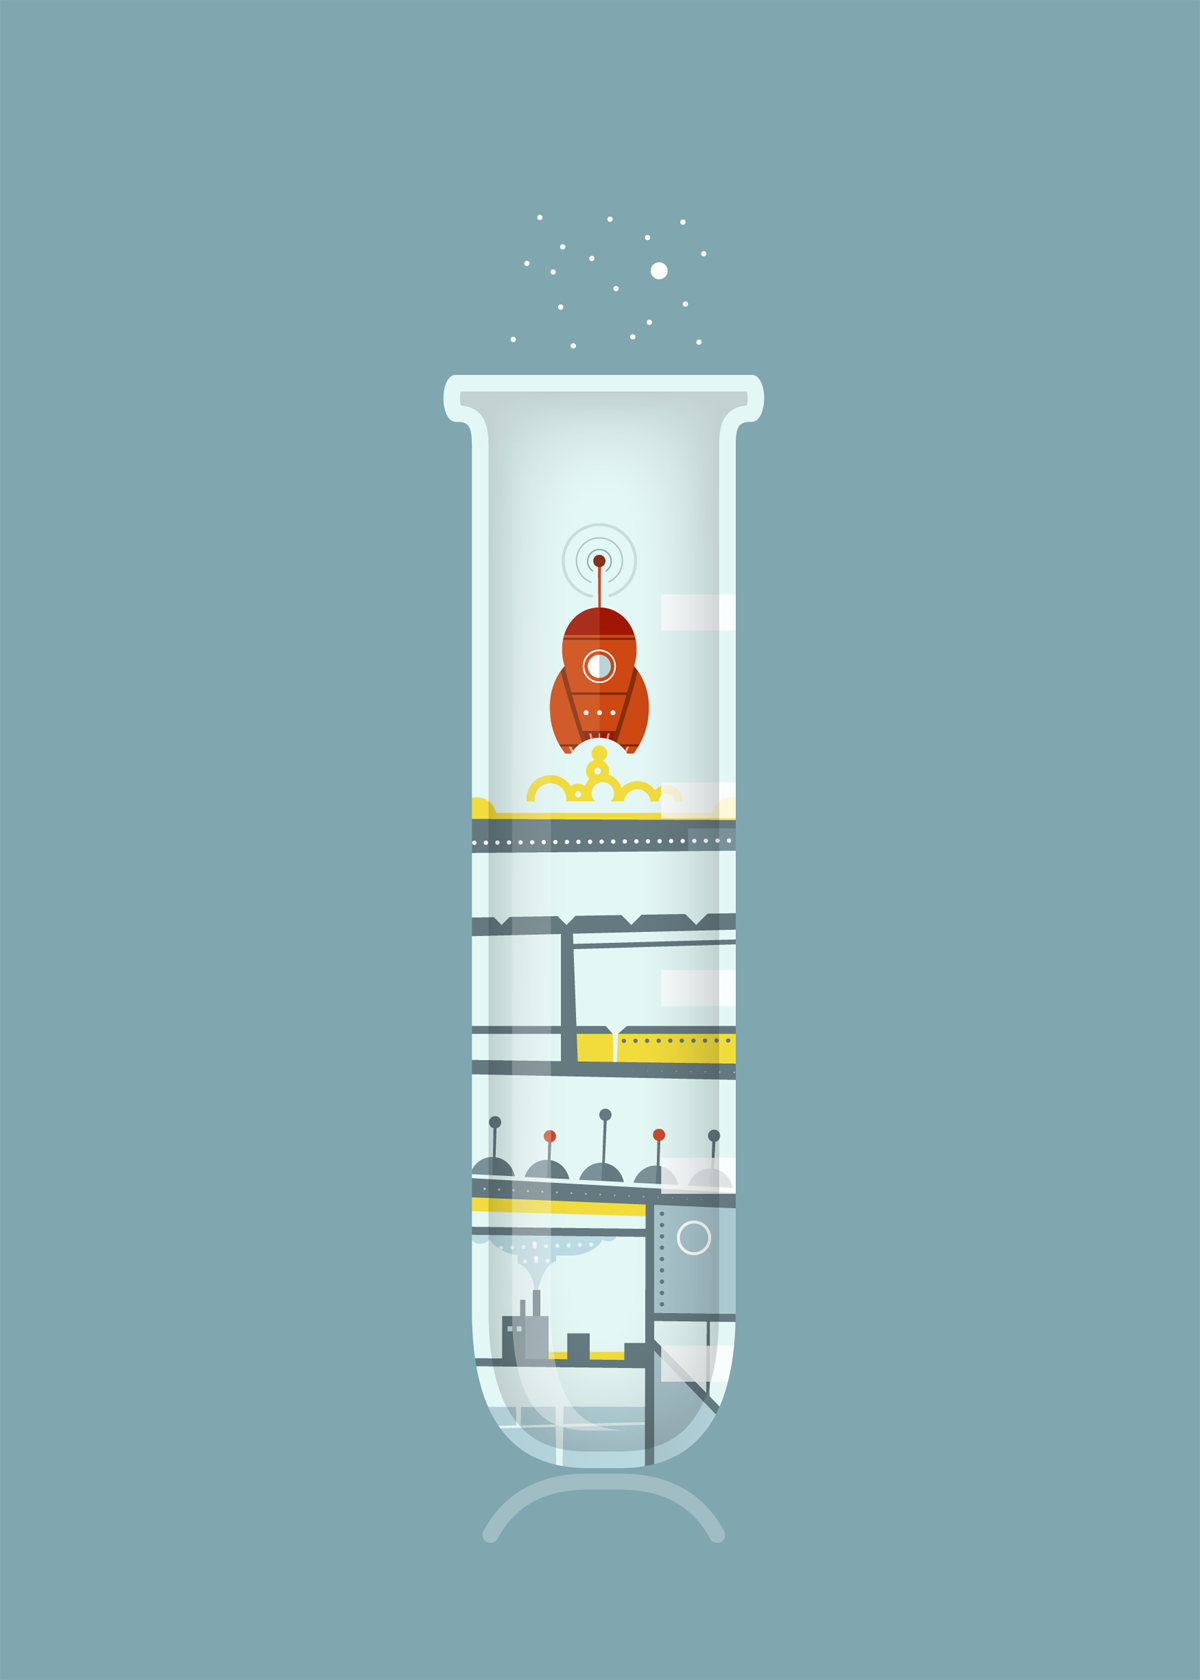
\includegraphics[width=0.42\textwidth]{endmatter/colophon.png}
\end{figure}

% If you don't want an image in the colophon:
% \vspace*{200pt}

\begin{center}
\parbox{200pt}{\lettrine[lines=3,slope=-2pt,nindent=-4pt]{\textcolor{SchoolColor}{T}}{his thesis was typeset} using \LaTeX, originally developed by Leslie Lamport and based on Donald Knuth's \TeX. The body text is set in 11 point Egenolff-Berner Garamond, a revival of Claude Garamont's humanist typeface. The above illustration, \textit{Science Experiment 02}, was created by Ben Schlitter and released under \href{http://creativecommons.org/licenses/by-nc-nd/3.0/}{\textsc{cc by-nc-nd 3.0}}. A template that can be used to format a PhD dissertation with this look \textit{\&} feel has been released under the permissive \textsc{agpl} license, and can be found online at \href{https://github.com/suchow/Dissertate}{github.com/suchow/Dissertate} or from its lead author, Jordan Suchow, at \href{mailto:suchow@post.harvard.edu}{suchow@post.harvard.edu}.}
\end{center}


\end{document}